% Chapter 5
\chapter{THỰC NGHIỆM VÀ ĐÁNH GIÁ}
\label{Chapter5}

Chương này báo cáo thực nghiệm trên CIC-IoT-2023 và ToN-IoT, gồm: thiết lập thực nghiệm, đánh giá phòng thủ, đánh giá bộ sinh, phát hiện free-rider, phân tích overhead, và bàn luận.

\section{Thiết lập thực nghiệm}

\subsection{Môi trường thực nghiệm}
\textbf{Phần cứng:} Toàn bộ thực nghiệm được thực hiện trên máy tính xách tay trang bị processor Apple M2 (8-core CPU, kiến trúc ARM64), bộ nhớ RAM 16 GB, không sử dụng GPU rời. Việc huấn luyện và suy luận mô hình đều chạy trên CPU thông qua PyTorch, phù hợp với mục tiêu đánh giá hiệu năng phòng thủ trong môi trường tài nguyên hạn chế, đặc trưng của các thiết bị edge IoT.

\textbf{Phần mềm:} Ngôn ngữ lập trình Python 3.11.6. Các thư viện chính: PyTorch 2.11.0 cho huấn luyện và suy luận mô hình học sâu; NumPy 1.24+ cho tính toán số; Pandas 2.0+ cho xử lý dữ liệu; scikit-learn 1.3+ cho các metric đánh giá; Matplotlib 3.7+ và Seaborn 0.12+ cho trực quan hóa. Mô hình sinh dữ liệu thách thức TabDDPM được xây dựng dựa trên thư viện diffusion models với kiến trúc MLP tùy chỉnh.

\textbf{Môi trường mô phỏng FL:} Hệ thống FL được xây dựng tùy chỉnh bằng Python, mô phỏng đầy đủ quy trình Federated Learning gồm: phân chia dữ liệu Non-IID theo phân phối Dirichlet, huấn luyện cục bộ trên từng client, tổng hợp tại server, và triển khai cả 9 phương pháp phòng thủ baseline. Môi trường mô phỏng cho phép kiểm soát hoàn toàn các biến số (tỉ lệ client độc hại, loại tấn công, seed ngẫu nhiên) nhằm đảm bảo so sánh công bằng giữa các phương pháp. Toàn bộ thực nghiệm sử dụng random seed cố định SEED = 42 để đảm bảo tính tái lập: np.random.seed(42) và torch.manual\_seed(42) được thiết lập trước mỗi kịch bản thực nghiệm.

\textbf{Ghi chú về mô phỏng:} Mô phỏng FL chạy tuần tự trên một máy đơn, mô phỏng hành vi của 20 client và 1 server trong cùng một tiến trình. Mặc dù thực tế FL chạy phân tán trên nhiều thiết bị, mô phỏng tuần tự là phương pháp chuẩn trong các nghiên cứu FL phòng thủ {[}1, 2, 5, 15, 16, 18, 19{]}, vì mục tiêu chính là đánh giá thuật toán phòng thủ (aggregation, filtering, scoring) chứ không phải hiệu năng giao tiếp mạng. Kết quả overhead thời gian (Mục 5.5) phản ánh chi phí tính toán của từng phương pháp, không bao gồm độ trễ mạng. Đây là thách thức của triển khai thực tế, nằm ngoài phạm vi đề tài.

\subsection{Cấu hình Federated Learning}
Cấu hình FL chung cho cả hai bộ dữ liệu: số client N = 20, số vòng lặp R = 20, batch size = 512, optimizer Adam (learning rate = $10^{-3}$), loss function Weighted Cross-Entropy, phân bổ dữ liệu Non-IID theo Dirichlet ($\alpha$ = 0,5). Mô hình IDS cho cả hai dataset là IoTAttackNet --- mạng MLP với kiến trúc input $\rightarrow$ 256 $\rightarrow$ 128 $\rightarrow$ 64 $\rightarrow$ num\_classes, sử dụng ReLU activation, BatchNorm, và Dropout (p = 0,3).

Các tham số được điều chỉnh theo từng bộ dữ liệu:

\begin{longtable}[]{@{}
  >{\raggedright\arraybackslash}p{(\linewidth - 4\tabcolsep) * \real{0.3642}}
  >{\raggedright\arraybackslash}p{(\linewidth - 4\tabcolsep) * \real{0.2243}}
  >{\raggedright\arraybackslash}p{(\linewidth - 4\tabcolsep) * \real{0.1567}}@{}}
\caption{Cấu hình thực nghiệm theo từng bộ dữ liệu} \\
\toprule\noalign{}
\begin{minipage}[b]{\linewidth}\centering
\textbf{Tham số}
\end{minipage} & \begin{minipage}[b]{\linewidth}\centering
\textbf{CIC-IoT-2023}
\end{minipage} & \begin{minipage}[b]{\linewidth}\centering
\textbf{ToN-IoT}
\end{minipage} \\
\midrule\noalign{}
\endfirsthead
%
\multicolumn{3}{c}{{\textit{(tiếp) Bảng 5.1}}} \\
\toprule\noalign{}
\begin{minipage}[b]{\linewidth}\centering
\textbf{Tham số}
\end{minipage} & \begin{minipage}[b]{\linewidth}\centering
\textbf{CIC-IoT-2023}
\end{minipage} & \begin{minipage}[b]{\linewidth}\centering
\textbf{ToN-IoT}
\end{minipage} \\
\midrule\noalign{}
\endhead
\bottomrule\noalign{}
\endlastfoot
Số đặc trưng / lớp & 39 / 34 & 10 / 10 \\
Local epochs (E) & 3 & 2 \\
Ngưỡng Trust-Score ($\theta_{T}$) & 0,6 & 0,5 \\
Số mẫu challenge & 200 & 500 \\
\end{longtable}

Tỉ lệ client độc hại được đánh giá ở bốn mức: 10\% (2 client), 20\% (4 client), 40\% (8 client), và 50\% (10 client), từ mức nhẹ đến mức khắc nghiệt nhất.

\subsection{Các phương pháp đối sánh}
DT-Guard được so sánh với chín phương pháp phòng thủ đại diện, phân thành ba nhóm:

\begin{itemize}
\item
  \textbf{Không phòng thủ:} FedAvg {[}9{]}
\item
  \textbf{Thống kê cổ điển:} Krum {[}2{]}, Median {[}18{]}, Trimmed Mean {[}18{]}, GeoMed {[}12{]}
\item
  \textbf{Phân tích nâng cao:} SignGuard {[}16{]}, ClipCluster {[}19{]}, LUP {[}5{]}, PoC {[}22{]}
\end{itemize}

\subsection{Các chỉ số đánh giá}
Ba chỉ số chính được sử dụng:

\begin{itemize}
\item
  \textbf{Accuracy:} Hiệu năng phát hiện xâm nhập của mô hình toàn cục trên tập kiểm tra.
\item
  \textbf{Detection Rate (DR):} Tỉ lệ client độc hại bị DT-Guard phát hiện và loại bỏ chính xác.
\item
  \textbf{False Positive Rate (FPR):} Tỉ lệ client lành tính bị loại nhầm.
\end{itemize}

\subsection{Kịch bản thực nghiệm}
Thực nghiệm gồm ba kịch bản:

Kịch bản A (Đánh giá hiệu năng phòng thủ): 5 loại tấn công (Backdoor, LIE, Min-Max, Min-Sum, MPAF) $\times$ 4 mức tỉ lệ malicious (10\%, 20\%, 40\%, 50\%) = 20 kịch bản trên mỗi dataset (CIC-IoT-2023 và ToN-IoT), tổng cộng 40 kịch bản.

Kịch bản B (Đánh giá bộ sinh dữ liệu thách thức): A/B Testing 5 mô hình sinh (TabDDPM, TabSyn, ForestDiffusion, CTGAN, WGAN-GP).

Kịch bản C (Đánh giá tính công bằng và phát hiện free-rider): 4 free-rider trong 20 client, so sánh 4 chiến lược tổng hợp.

\subsection{Phân tích khám phá dữ liệu (EDA)}
\label{sec:eda}
Trước khi thực hiện các kịch bản chính, phần này phân tích chi tiết đặc điểm của hai bộ dữ liệu nhằm làm rõ năm yếu tố ảnh hưởng trực tiếp đến hiệu năng phòng thủ: phân phối lớp tổng thể, thống kê mô tả đặc trưng, phân phối giá trị đặc trưng, label skew và feature skew sau khi phân chia Dirichlet.

\subsubsection{Phân phối lớp tổng thể trước khi chia train--test}
Bảng \ref{tab:cic_class_dist} thống kê phân phối mẫu theo danh mục tấn công trên \textit{toàn bộ} dataset CIC-IoT-2023 gốc (46,7 triệu mẫu, gộp 63 file CSV, theo công bố chính thức {[}11{]}); thực nghiệm sử dụng slice Merged01.csv (712.311 mẫu) làm tập đại diện vì phân phối tương đối được bảo toàn (DDoS $\approx$72,3\% so với 72,82\% trên toàn bộ). Dữ liệu mất cân bằng cực kỳ nghiêm trọng: DDoS chiếm 72,82\%, trong khi BruteForce chỉ chiếm 0,03\%---tỷ lệ chênh lệch $\sim$2.600$\times$.

\begin{table}[H]
\centering
\caption{Phân phối mẫu theo danh mục tấn công trong CIC-IoT-2023 (toàn bộ dataset gốc) {[}11{]}}
\label{tab:cic_class_dist}
\small
\begin{tabular}{|l|r|r|}
\hline
\textbf{Danh mục} & \textbf{Số dòng} & \textbf{Tỷ lệ (\%)} \\
\hline
DDoS & 33.984.560 & 72,82 \\
\hline
DoS & 8.090.738 & 17,34 \\
\hline
Mirai & 2.634.124 & 5,64 \\
\hline
Benign & 1.098.195 & 2,35 \\
\hline
Spoofing & 486.504 & 1,04 \\
\hline
Reconnaissance & 354.565 & 0,76 \\
\hline
Web-based & 24.829 & 0,05 \\
\hline
BruteForce & 13.064 & 0,03 \\
\hline
\textbf{Tổng} & \textbf{46.686.579} & \textbf{100,00} \\
\hline
\end{tabular}
\end{table}

Bảng \ref{tab:ton_iot_class_dist} thống kê phân phối ToN-IoT (toàn bộ dataset đã tiền xử lý). Đặc thù nổi bật: Normal chiếm 65\%, 8 lớp tấn công có $\sim$20.000 mẫu mỗi lớp, MITM chỉ 1.042 mẫu---mất cân bằng kiểu \textit{one-vs-many}.

\begin{table}[H]
\centering
\caption{Phân phối mẫu theo loại tấn công trong ToN-IoT {[}10{]}}
\label{tab:ton_iot_class_dist}
\small
\begin{tabular}{|l|r|r|}
\hline
\textbf{Loại} & \textbf{Số mẫu} & \textbf{Tỷ lệ (\%)} \\
\hline
Normal & 300.000 & 65,07 \\
\hline
Scanning & 20.000 & 4,34 \\
\hline
DoS & 20.000 & 4,34 \\
\hline
DDoS & 20.000 & 4,34 \\
\hline
Ransomware & 20.000 & 4,34 \\
\hline
Backdoor & 20.000 & 4,34 \\
\hline
Injection & 20.000 & 4,34 \\
\hline
XSS & 20.000 & 4,34 \\
\hline
Password & 20.000 & 4,34 \\
\hline
MITM & 1.042 & 0,23 \\
\hline
\textbf{Tổng} & \textbf{461.042} & \textbf{100,00} \\
\hline
\end{tabular}
\end{table}

Hai dạng mất cân bằng này (\textit{long-tail} ở CIC-IoT-2023 và \textit{one-vs-many} ở ToN-IoT) là cơ sở để áp dụng Weighted Cross-Entropy Loss (Mục~\ref{subsec:wce_loss}) và là nguồn gốc tự nhiên của \textit{label skew} sau khi phân chia Dirichlet (chi tiết tại Mục~\ref{subsec:eda_dirichlet}).

\subsubsection{Thống kê mô tả đặc trưng}
Bảng \ref{tab:cic_iot_feature_stats} thống kê đầy đủ 39 đặc trưng của CIC-IoT-2023, chia thành 5 nhóm: thông tin header mạng (4), cờ TCP (7), số lượng cờ (4), chỉ báo giao thức (15) và thống kê gói tin (9). Phần lớn đặc trưng chỉ báo giao thức (Telnet, SSH, IRC, SMTP, IGMP, DHCP) có giá trị trung bình $\approx 0$, cho thấy chúng hiếm khi xuất hiện trong lưu lượng IoT. Các đặc trưng liên tục như Variance (std $= 411{,}9$K) và Rate (max $= 5{,}2$M) trải rất rộng, phản ánh sự đa dạng mạnh của lưu lượng. Đối với ToN-IoT, dữ liệu đã được chuẩn hoá StandardScaler trước khi công bố nên 10 đặc trưng đều nằm trong dải chuẩn (mean$\approx$0, var$\in[0{,}03; 0{,}13]$); thống kê chi tiết được trình bày gián tiếp qua phân phối ở Mục~\ref{subsec:eda_value_dist}.

\begin{footnotesize}
\begin{longtable}{|l|l|r|r|r|r|}
\caption{Thống kê mô tả 39 đặc trưng CIC-IoT-2023 ($n = 712{.}311$ mẫu)} \label{tab:cic_iot_feature_stats} \\
\hline
\textbf{Đặc trưng} & \textbf{Loại} & \textbf{Mean} & \textbf{Std} & \textbf{Min} & \textbf{Max} \\
\hline
\endfirsthead
\hline
\textbf{Đặc trưng} & \textbf{Loại} & \textbf{Mean} & \textbf{Std} & \textbf{Min} & \textbf{Max} \\
\hline
\endhead
\multicolumn{6}{|l|}{\textit{Thông tin header mạng}} \\
\hline
Header\_Length & Liên tục & 13,76 & 8,72 & 0 & 60 \\
\hline
Protocol Type & Phân loại & 9,09 & 9,08 & 0 & 47 \\
\hline
Time\_To\_Live & Liên tục & 66,53 & 14,38 & 0 & 255 \\
\hline
Rate & Liên tục & 28,4K & 30,2K & 0,001 & 5,2M \\
\hline
\multicolumn{6}{|l|}{\textit{Cờ TCP}} \\
\hline
fin\_flag\_number & Nhị phân & 0,088 & 0,280 & 0 & 1 \\
\hline
syn\_flag\_number & Nhị phân & 0,207 & 0,400 & 0 & 1 \\
\hline
rst\_flag\_number & Nhị phân & 0,093 & 0,284 & 0 & 1 \\
\hline
psh\_flag\_number & Nhị phân & 0,094 & 0,277 & 0 & 1 \\
\hline
ack\_flag\_number & Nhị phân & 0,130 & 0,317 & 0 & 1 \\
\hline
ece\_flag\_number & Nhị phân & $\approx$0 & 0,002 & 0 & 0,6 \\
\hline
cwr\_flag\_number & Nhị phân & $\approx$0 & 0,002 & 0 & 0,6 \\
\hline
\multicolumn{6}{|l|}{\textit{Số lượng cờ (0--100)}} \\
\hline
ack\_count & Đếm & 9,87 & 28,05 & 0 & 100 \\
\hline
syn\_count & Đếm & 20,42 & 39,92 & 0 & 100 \\
\hline
fin\_count & Đếm & 8,66 & 28,01 & 0 & 100 \\
\hline
rst\_count & Đếm & 9,22 & 28,30 & 0 & 100 \\
\hline
\multicolumn{6}{|l|}{\textit{Chỉ báo giao thức}} \\
\hline
HTTP & Nhị phân & 0,050 & 0,214 & 0 & 1 \\
\hline
HTTPS & Nhị phân & 0,059 & 0,220 & 0 & 1 \\
\hline
DNS & Nhị phân & 0,003 & 0,022 & 0 & 1 \\
\hline
Telnet & Nhị phân & $\approx$0 & 0,001 & 0 & 0,3 \\
\hline
SMTP & Nhị phân & $\approx$0 & 0,001 & 0 & 0,4 \\
\hline
SSH & Nhị phân & $\approx$0 & 0,008 & 0 & 1 \\
\hline
IRC & Nhị phân & $\approx$0 & 0,001 & 0 & 0,2 \\
\hline
TCP & Nhị phân & 0,576 & 0,485 & 0 & 1 \\
\hline
UDP & Nhị phân & 0,217 & 0,401 & 0 & 1 \\
\hline
DHCP & Nhị phân & $\approx$0 & 0,005 & 0 & 0,5 \\
\hline
ARP & Nhị phân & 0,003 & 0,019 & 0 & 1 \\
\hline
ICMP & Nhị phân & 0,163 & 0,366 & 0 & 1 \\
\hline
IGMP & Nhị phân & $\approx$0 & 0,001 & 0 & 0,2 \\
\hline
IPv & Nhị phân & 0,997 & 0,019 & 0 & 1 \\
\hline
LLC & Nhị phân & 0,997 & 0,019 & 0 & 1 \\
\hline
\multicolumn{6}{|l|}{\textit{Thống kê gói tin}} \\
\hline
Tot sum & Liên tục & 10,9K & 16,8K & 60 & 239,4K \\
\hline
Min & Liên tục & 79,88 & 106,88 & 42 & 3,0K \\
\hline
Max & Liên tục & 222,50 & 586,94 & 54 & 30,5K \\
\hline
AVG & Liên tục & 130,90 & 227,67 & 48,4 & 5,4K \\
\hline
Std & Liên tục & 41,12 & 181,58 & 0 & 9,5K \\
\hline
Tot size & Liên tục & 130,90 & 227,67 & 48,4 & 5,4K \\
\hline
IAT & Liên tục & 0,002 & 0,883 & 0 & 741 \\
\hline
Number & Đếm & 95,51 & 19,56 & 1 & 100 \\
\hline
Variance & Liên tục & 34,7K & 411,9K & 0 & 90,9M \\
\hline
\end{longtable}
\end{footnotesize}

\subsubsection{Phân phối giá trị đặc trưng}
\label{subsec:eda_value_dist}
Hình \ref{fig:cic_iot_feature_dist} minh họa phân phối giá trị của 8 đặc trưng liên tục đại diện trong CIC-IoT-2023. Đa số đặc trưng có phân phối lệch phải nặng: phần lớn mẫu tập trung ở giá trị thấp, trong khi một tỷ lệ nhỏ có giá trị rất cao---dấu hiệu của tấn công burst tạo outlier. Nhiều đặc trưng (Std, Variance, IAT) tập trung ở giá trị 0, phản ánh thực tế rằng nhiều flow ngắn có tất cả gói tin cùng kích thước. Một số đặc trưng như Rate và Variance có giá trị trải dài qua nhiều cấp độ lớn, cho thấy lưu lượng IoT rất đa dạng và đòi hỏi chuẩn hóa phù hợp.

\begin{figure}[H]
    \centering
    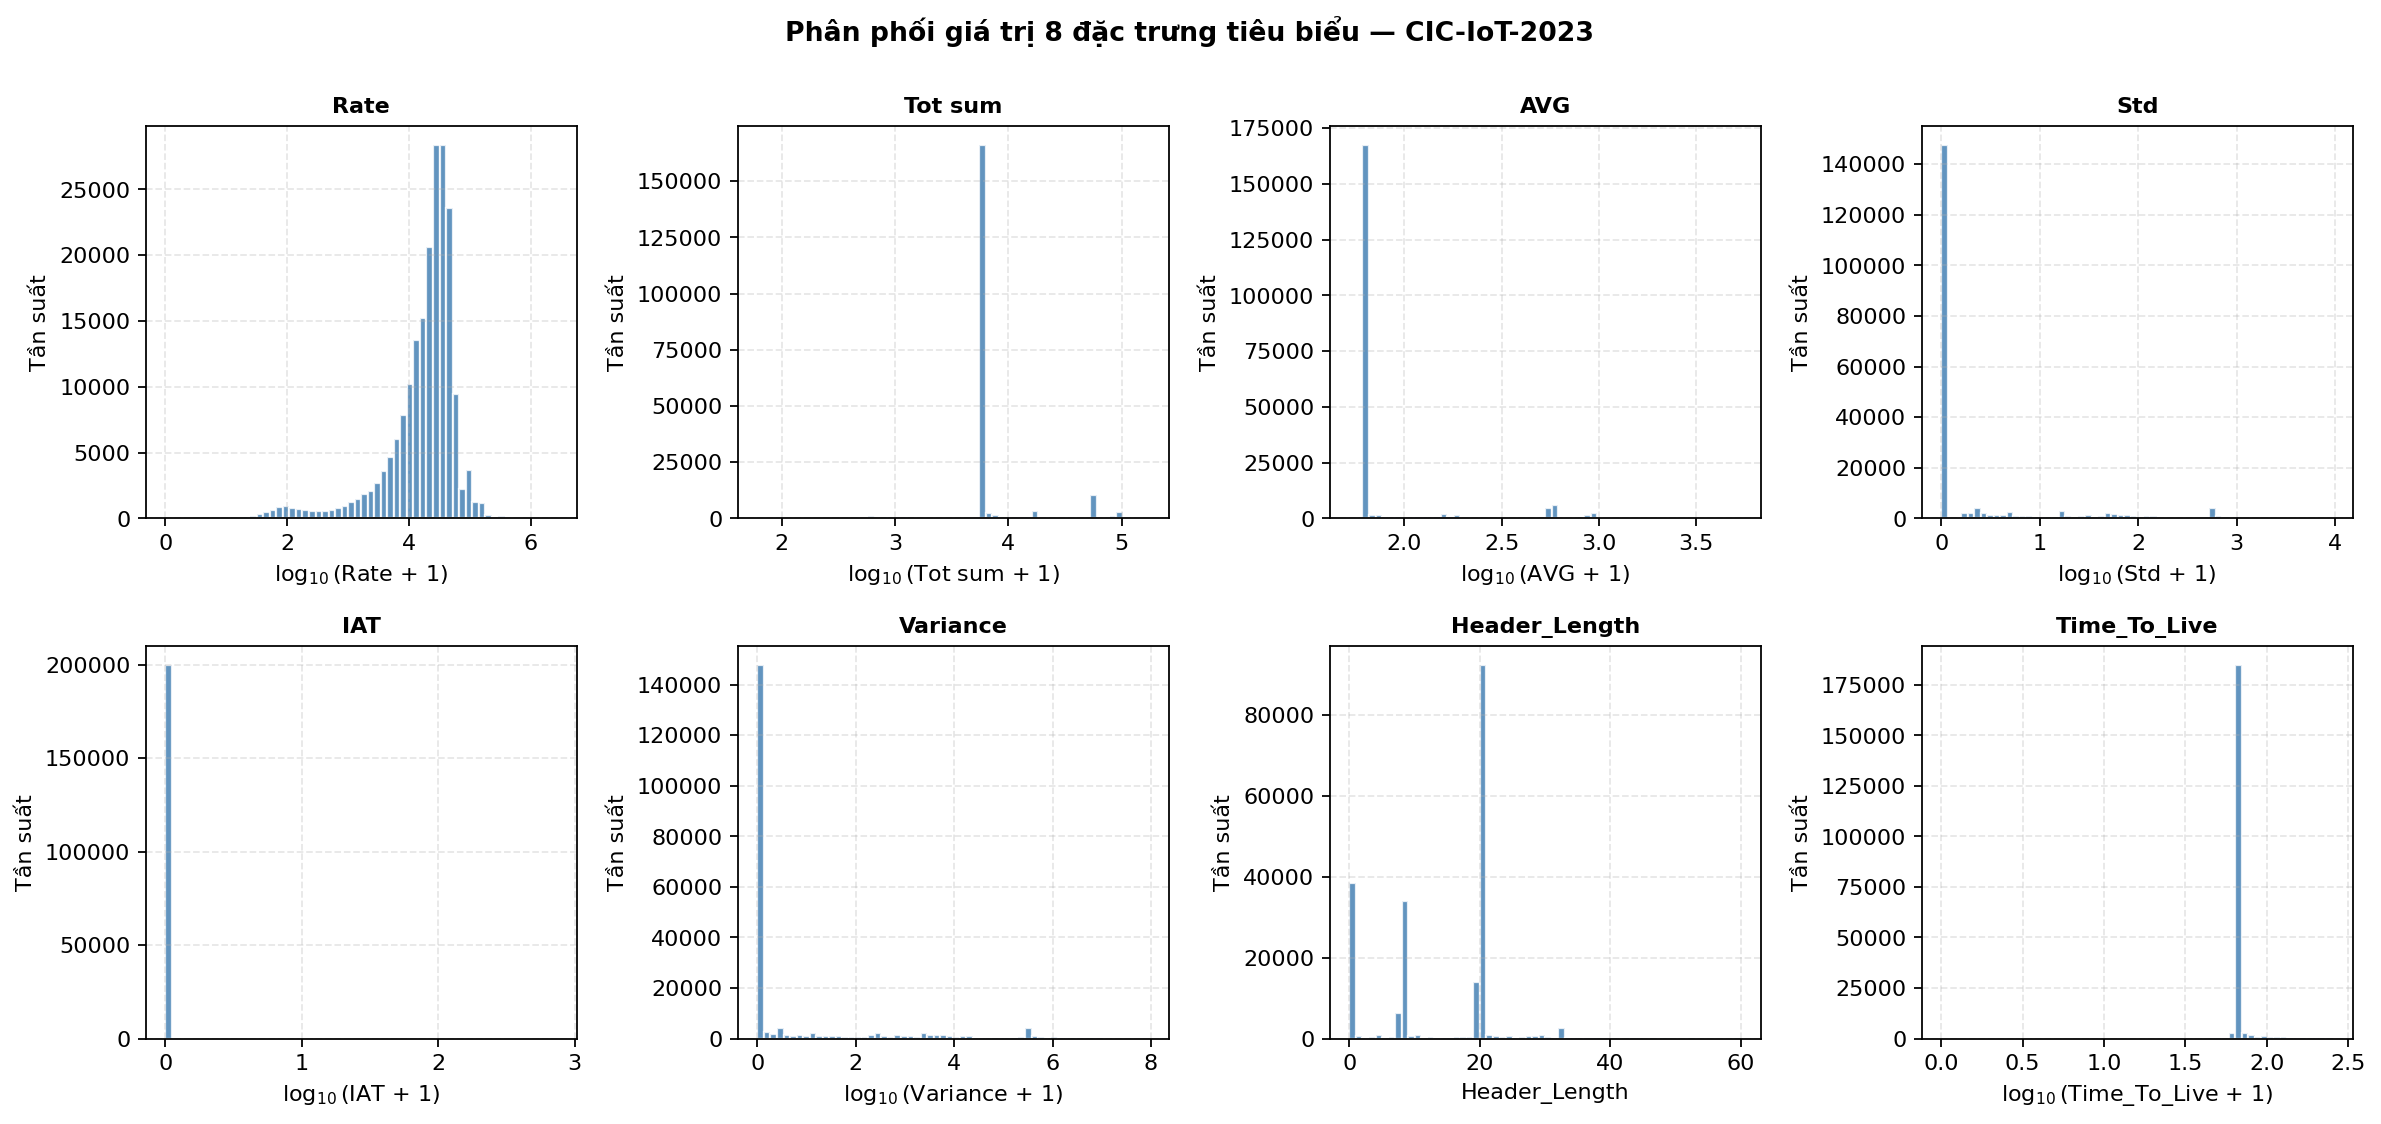
\includegraphics[width=0.90\linewidth]{Figures/fig_5_1_cic_iot_feature_dist.png}
    \caption{Phân phối giá trị 8 đặc trưng liên tục đại diện trong CIC-IoT-2023}
    \label{fig:cic_iot_feature_dist}
\end{figure}

Hình \ref{fig:ton_iot_feature_dist} minh họa phân phối 10 đặc trưng ToN-IoT sau chuẩn hóa StandardScaler. So với CIC-IoT-2023, các đặc trưng có phân phối đa đỉnh (multi-modal), mỗi đỉnh tương ứng với một nhóm loại tấn công. Đặc trưng có khoảng giá trị hẹp hơn và phân phối ổn định hơn, phản ánh việc đã chọn lọc 10 đặc trưng quan trọng nhất từ 44 đặc trưng ban đầu.

\begin{figure}[H]
    \centering
    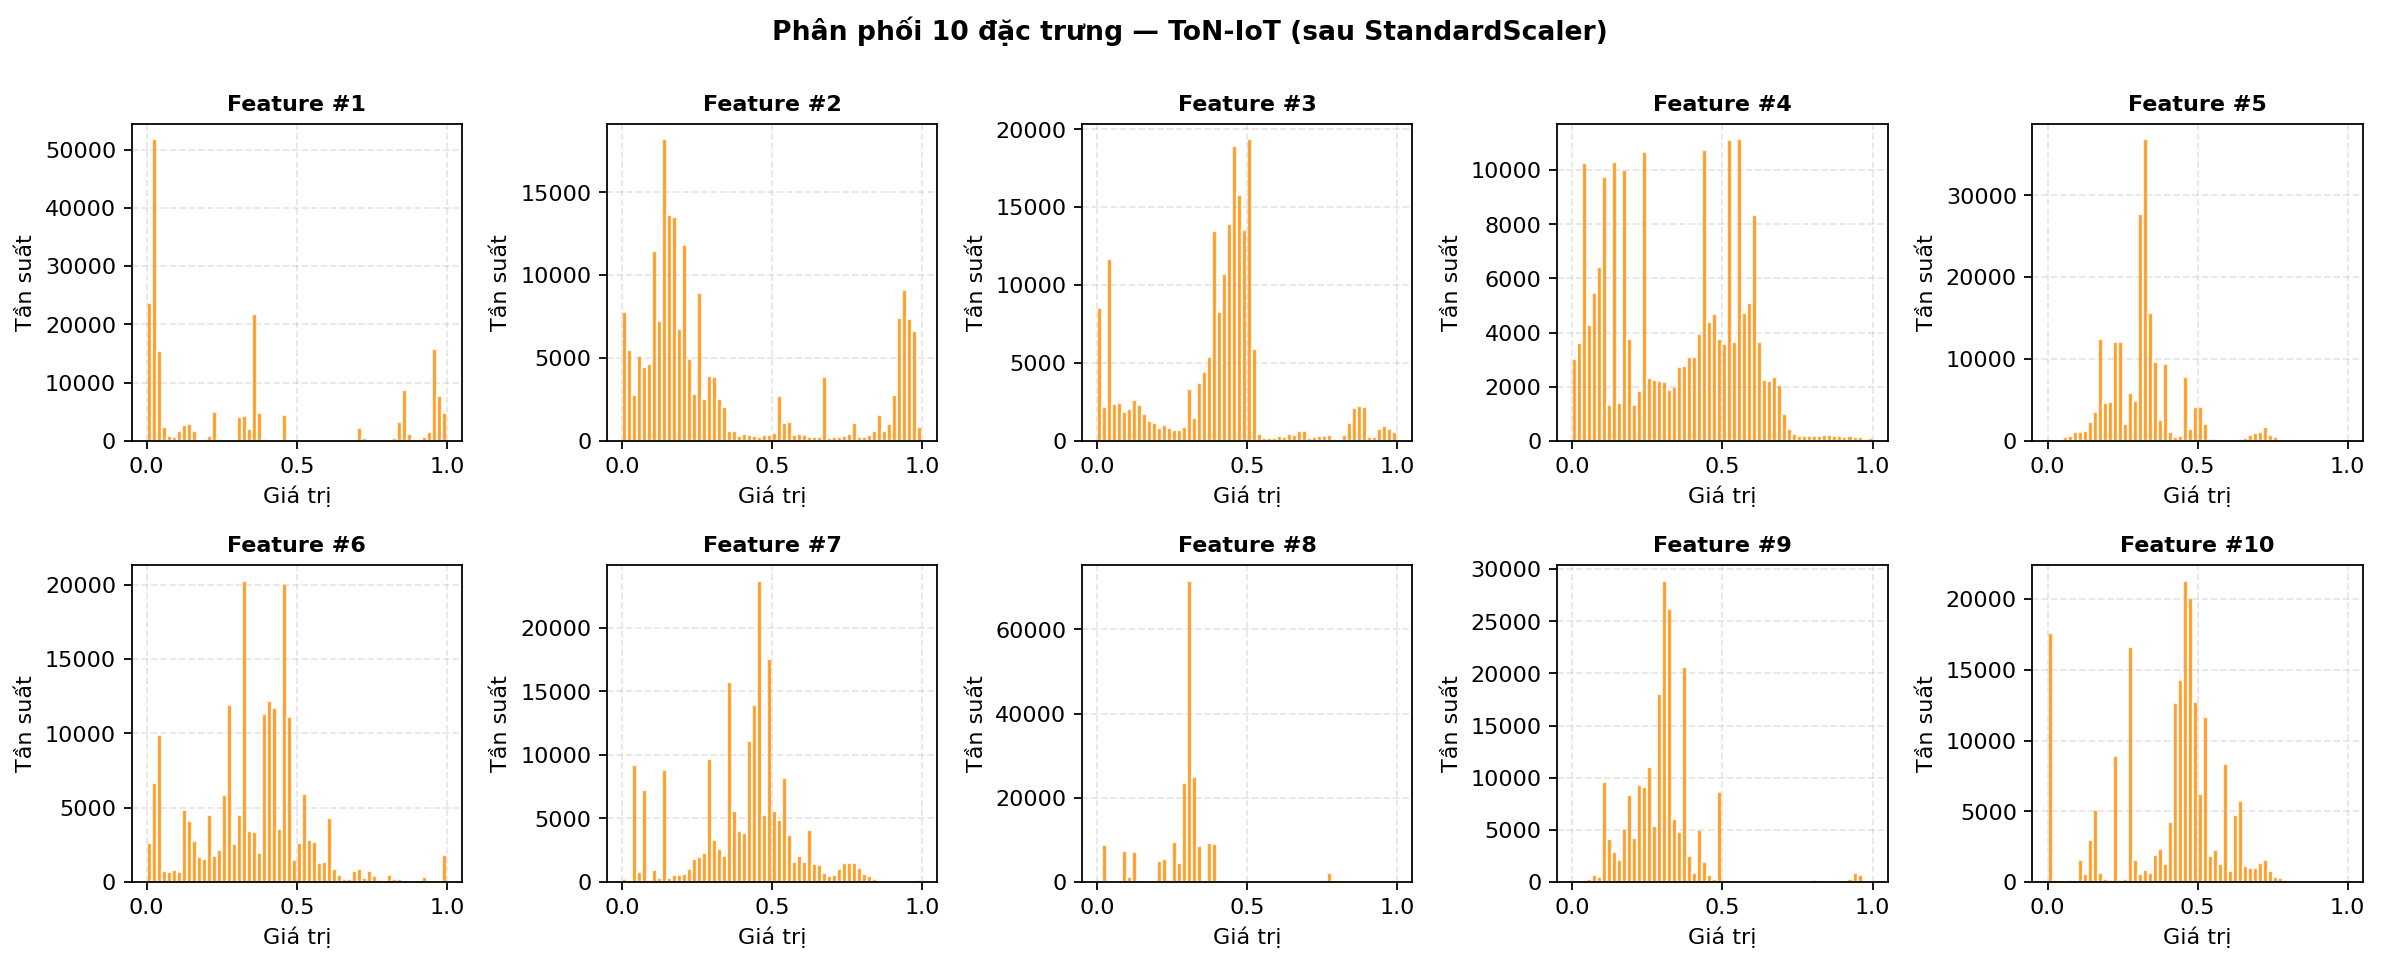
\includegraphics[width=0.90\linewidth]{Figures/fig_5_2_ton_iot_feature_dist.png}
    \caption{Phân phối giá trị 10 đặc trưng trong ToN-IoT (sau StandardScaler)}
    \label{fig:ton_iot_feature_dist}
\end{figure}

\subsubsection{Phân chia Dirichlet và mức độ Non-IID (label skew)}
\label{subsec:eda_dirichlet}
Hình \ref{fig:cic_iot_dirichlet_split} và Hình \ref{fig:ton_iot_dirichlet_split} trực quan hóa kết quả phân chia Dirichlet trên cả hai dataset với 10 client. Khi $\alpha=0{,}1$, mỗi client gần như chỉ chứa 1--2 lớp (label skew cực đoan); khi $\alpha=0{,}5$, phân phối đa dạng hơn nhưng vẫn chênh lệch đáng kể.

\textbf{CIC-IoT-2023 (Hình \ref{fig:cic_iot_dirichlet_split}):} Với $\alpha=0{,}1$, một số client bị chi phối bởi một loại tấn công DDoS/DoS duy nhất chiếm trên 60\% mẫu (ví dụ DDOS-UDP\_FLOOD 62\% ở C1, DOS-SYN\_FLOOD 78\% ở C4, DDOS-TCP\_FLOOD 64\% ở C8), trong khi các client khác chỉ nhận được dưới 3.000 mẫu (C10 chỉ 1.414 mẫu). Sự chênh lệch số mẫu giữa client lớn nhất (C5, $\sim$48 nghìn) và nhỏ nhất (C10) lên đến $\sim$34$\times$. Với $\alpha=0{,}5$, sự phân tán giảm rõ rệt: lớp tấn công đứng đầu ở mỗi client chỉ chiếm 15--43\% (không client nào còn vượt 50\%), và độ chênh số mẫu thu hẹp xuống $\sim$5$\times$. Các lớp thiểu số (BruteForce, XSS, Web-based) gần như không hiển thị trên biểu đồ do tỷ lệ quá nhỏ, cho thấy 34 lớp tấn công tạo ra Non-IID phức tạp hơn nhiều so với bộ dữ liệu chỉ có 10 lớp.

\textbf{ToN-IoT (Hình \ref{fig:ton_iot_dirichlet_split}):} Với $\alpha=0{,}1$, một số client gần như chỉ chứa một lớp (ví dụ C8 có 99,6\% là DoS, C4 có 93,7\% là Normal, C10 có 86\% là XSS, C2 có 82\% là Ransomware). Sự chênh lệch số mẫu giữa client lớn nhất (C4, $\sim$151 nghìn) và nhỏ nhất (C3, 476 mẫu) lên đến $\sim$318$\times$. Với $\alpha=0{,}5$, phân phối cân bằng hơn nhưng Normal vẫn chiếm đa số ở 6/10 client (39--78\%), độ chênh số mẫu giảm xuống $\sim$15$\times$. MITM---lớp hiếm nhất---hoàn toàn vắng mặt ở 5/10 client khi $\alpha=0{,}1$ và chỉ xuất hiện thưa thớt khi $\alpha=0{,}5$, tạo thách thức lớn cho phát hiện tấn công hiếm trong môi trường phân tán.

\begin{figure}[H]
    \centering
    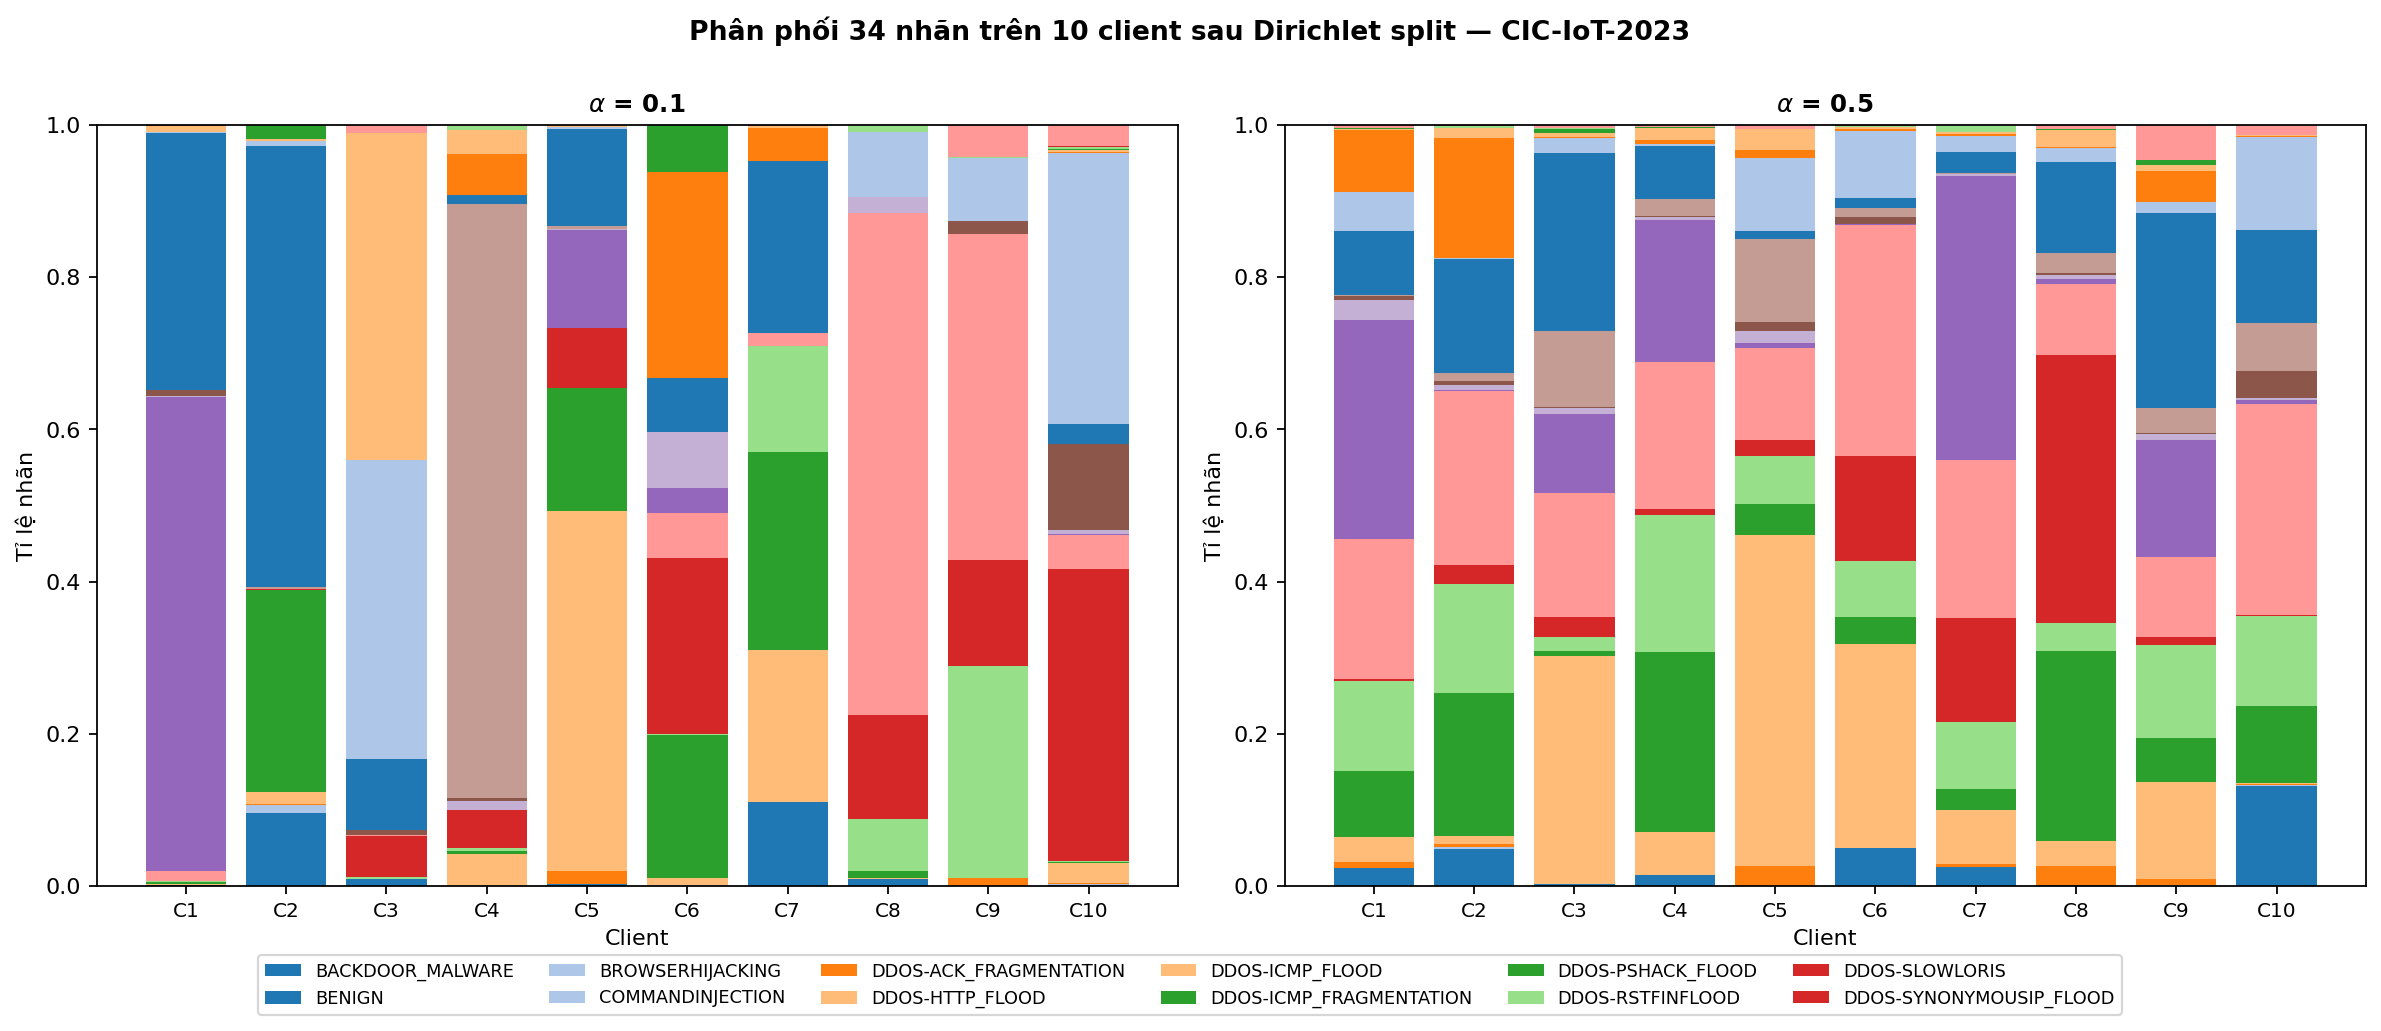
\includegraphics[width=0.95\linewidth]{Figures/fig_5_3_cic_iot_dirichlet_split.png}
    \caption{Phân phối 34 nhãn trên 10 client sau Dirichlet splitting -- CIC-IoT-2023 (trái: $\alpha=0{,}1$, phải: $\alpha=0{,}5$)}
    \label{fig:cic_iot_dirichlet_split}
\end{figure}

\begin{figure}[H]
    \centering
    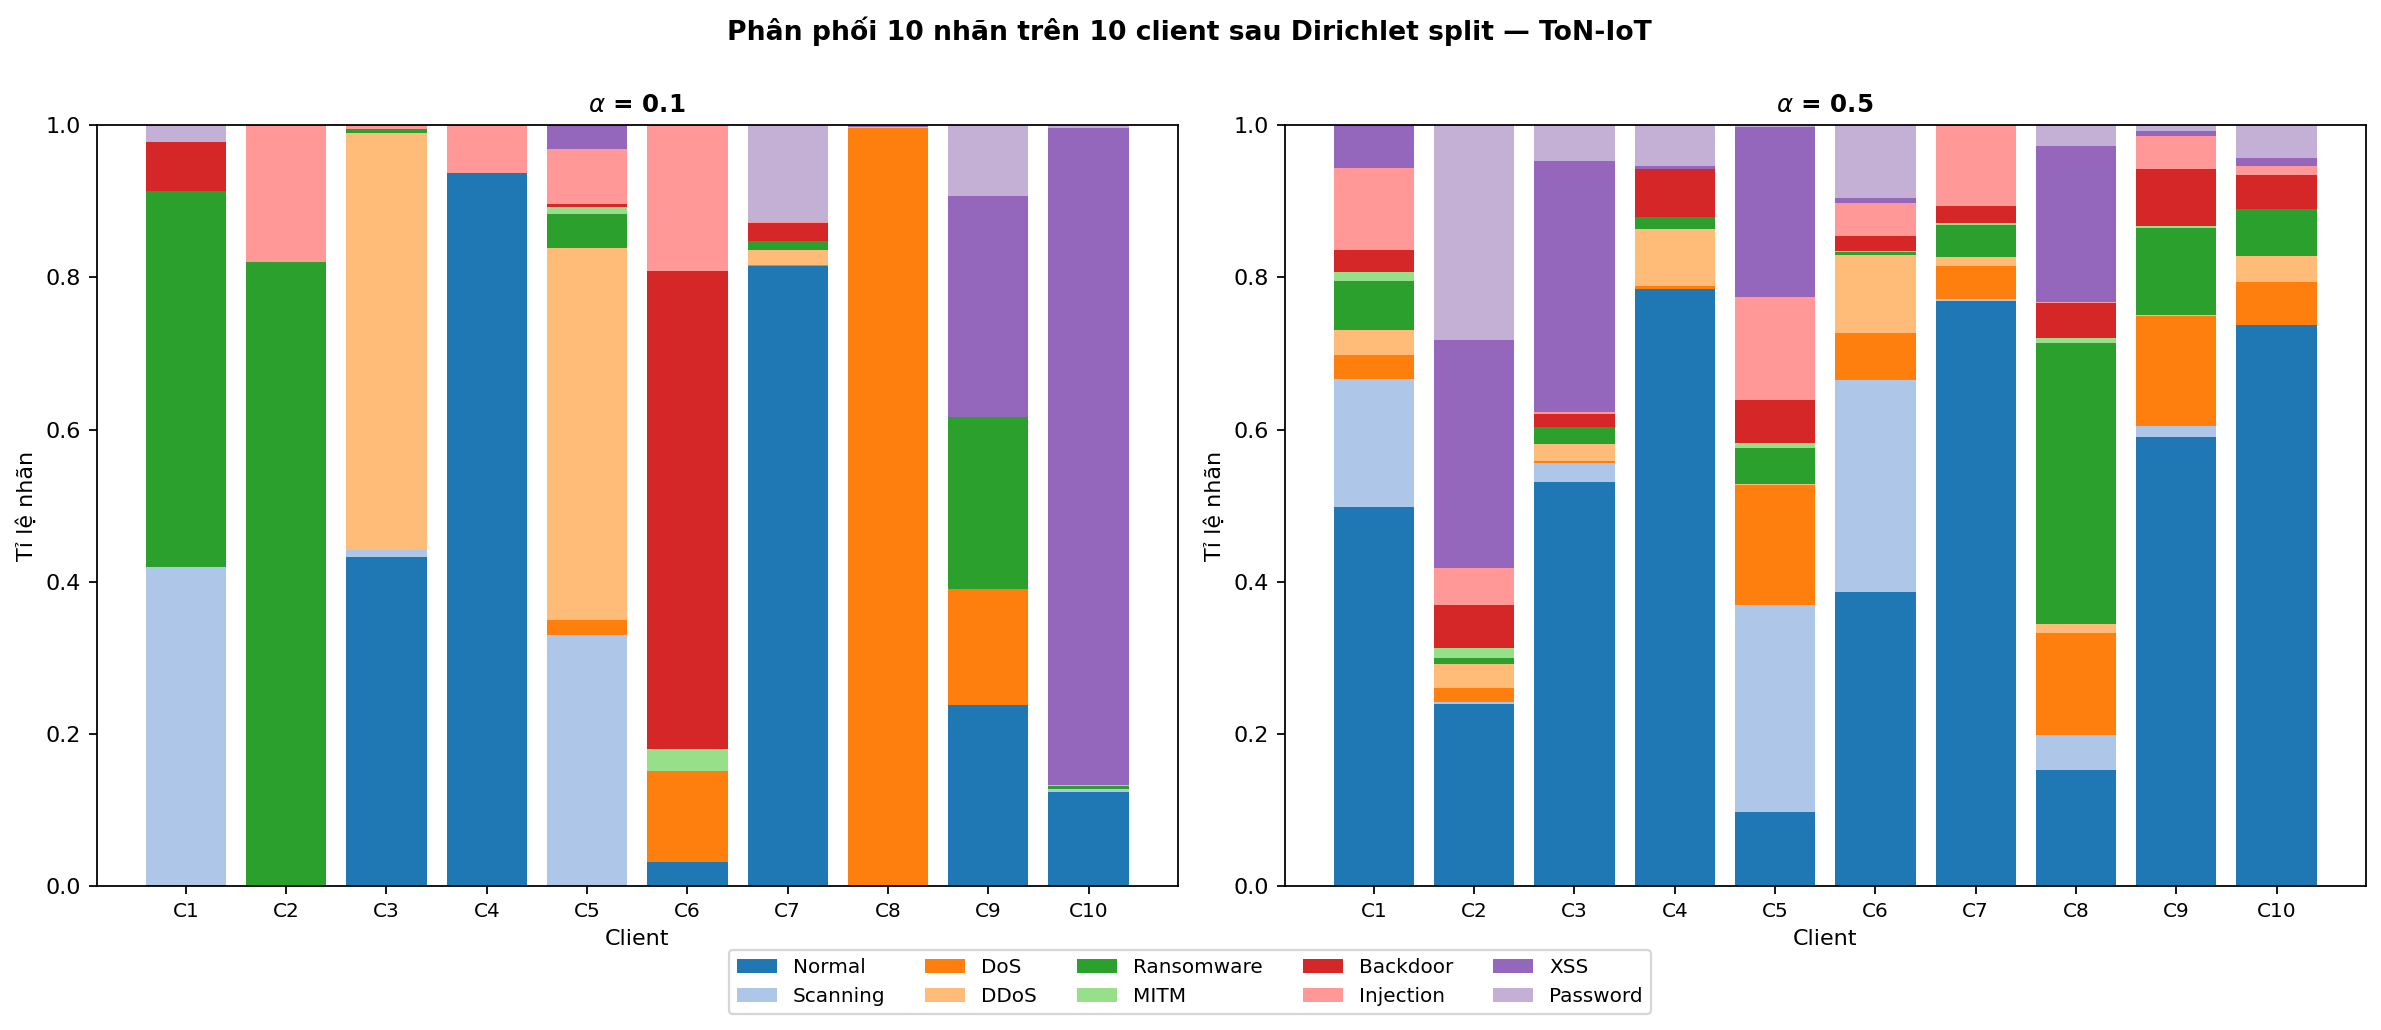
\includegraphics[width=0.95\linewidth]{Figures/fig_5_4_ton_iot_dirichlet_split.png}
    \caption{Phân phối 10 nhãn trên 10 client sau Dirichlet splitting -- ToN-IoT (trái: $\alpha=0{,}1$, phải: $\alpha=0{,}5$)}
    \label{fig:ton_iot_dirichlet_split}
\end{figure}

\subsubsection{Phân phối giá trị đặc trưng theo client (feature skew)}
\label{subsec:eda_feature_skew}
Bên cạnh \textit{label skew}, Dirichlet splitting còn gây ra \textit{feature skew} (Mục 3.1.3): cùng một đặc trưng nhưng phân phối giá trị giữa các client khác nhau rõ rệt do mỗi client tập trung vào tập lớp riêng. Hình \ref{fig:cic_iot_feat_skew} và Hình \ref{fig:ton_iot_feat_skew} minh hoạ hiện tượng này bằng boxplot của các đặc trưng tiêu biểu trên 10 client sau khi split.

\textbf{Lý do chọn đặc trưng minh hoạ.} Không gian đặc trưng quá lớn để vẽ toàn bộ (39 cột với CIC-IoT-2023, 10 cột với ToN-IoT), nên mỗi dataset chọn hai đặc trưng tiêu biểu là biến liên tục có dải giá trị rộng. Trên CIC-IoT-2023, hai đặc trưng được chọn là \texttt{Rate} (tốc độ gói tin, dùng log-scale do dải 0,001--5,2M) và \texttt{Header\_Length} (độ dài header IP/TCP, 0--60 byte với hai mode tự nhiên)---hai khía cạnh khác nhau (cường độ và cấu trúc giao thức) cùng phân biệt rõ giữa các họ tấn công. Trên ToN-IoT, do dữ liệu đã ẩn danh tên cột gốc sau feature selection và StandardScaler, tiêu chí khách quan là chọn hai cột có phương sai cao nhất: \texttt{feature\_0} (var = 0,130) và \texttt{feature\_1} (var = 0,103).

\textbf{CIC-IoT-2023 (Hình \ref{fig:cic_iot_feat_skew}):} Với \texttt{Rate}, khi $\alpha=0{,}1$ trung vị giữa các client chênh lệch khoảng 8$\times$ ($\approx$ 0,9 bậc của log): một số client có trung vị $\sim$3.800 pkt/s, trong khi client khác đạt $\sim$29.000 pkt/s; khi tăng lên $\alpha=0{,}5$ độ chênh thu hẹp xuống chỉ $\sim$1,7$\times$ và phân phối giữa các client trở nên đồng đều hơn nhiều. Với \texttt{Header\_Length}, hiện tượng skew thể hiện ở dạng khác: với $\alpha=0{,}1$ một số client có trung vị tập trung quanh 8 byte (chứa chủ yếu DDoS-ICMP), một số client khác quanh 20 byte (chứa chủ yếu DDoS-TCP/HTTP), và có client phân tán rộng từ 0 đến 28 byte; với $\alpha=0{,}5$ phần lớn client hội tụ về vùng trung vị 20 byte với IQR đa dạng nhưng vẫn còn vài client lệch xuống 8 byte. Cả hai đặc trưng đều cho thấy: $\alpha$ càng nhỏ thì feature skew càng rõ rệt.

\textbf{ToN-IoT (Hình \ref{fig:ton_iot_feat_skew}):} Trên hai cột \texttt{feature\_0} và \texttt{feature\_1} (hai cột có phương sai cao nhất sau StandardScaler), các boxplot cho thấy phân phối lệch giữa các client: với $\alpha=0{,}1$ trung vị dao động trong dải $\sim$0,35 (từ $\sim$0,001 đến $\sim$0,35), một số client có phân phối tập trung quanh một mode trong khi client khác phân tán rộng hơn. Với $\alpha=0{,}5$ phân phối giữa các client trở nên đồng đều hơn (dải trung vị thu hẹp xuống $\sim$0,1) nhưng vẫn còn vài client lệch trung vị.

\begin{figure}[H]
    \centering
    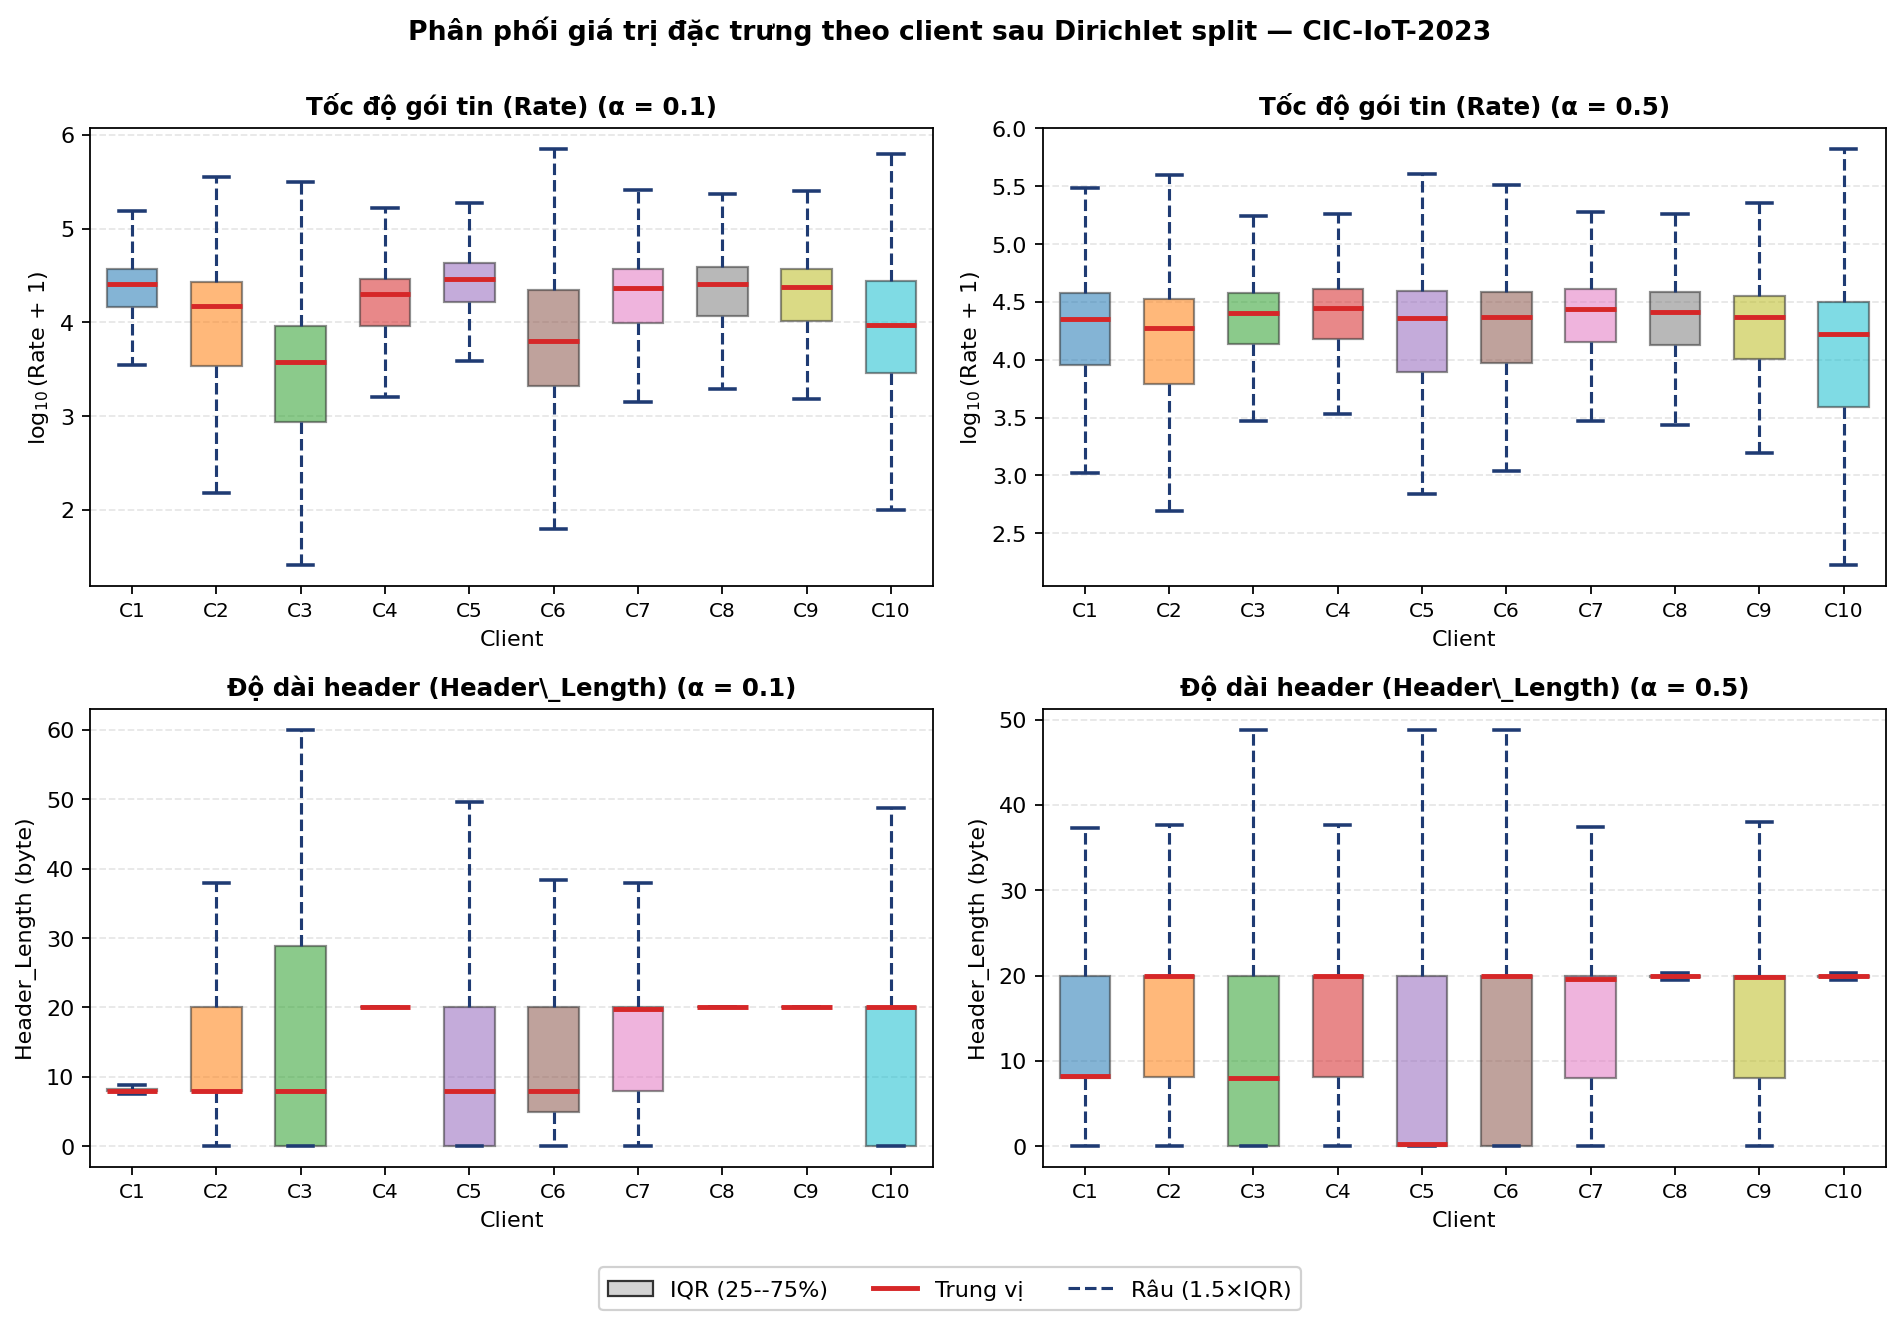
\includegraphics[width=0.95\linewidth]{Figures/fig_5_5_cic_iot_feature_skew_per_client.png}
    \caption{Phân phối giá trị đặc trưng theo client sau Dirichlet split -- CIC-IoT-2023 (\texttt{Rate} log-scale và \texttt{Header\_Length}; trái: $\alpha=0{,}1$, phải: $\alpha=0{,}5$)}
    \label{fig:cic_iot_feat_skew}
\end{figure}

\begin{figure}[H]
    \centering
    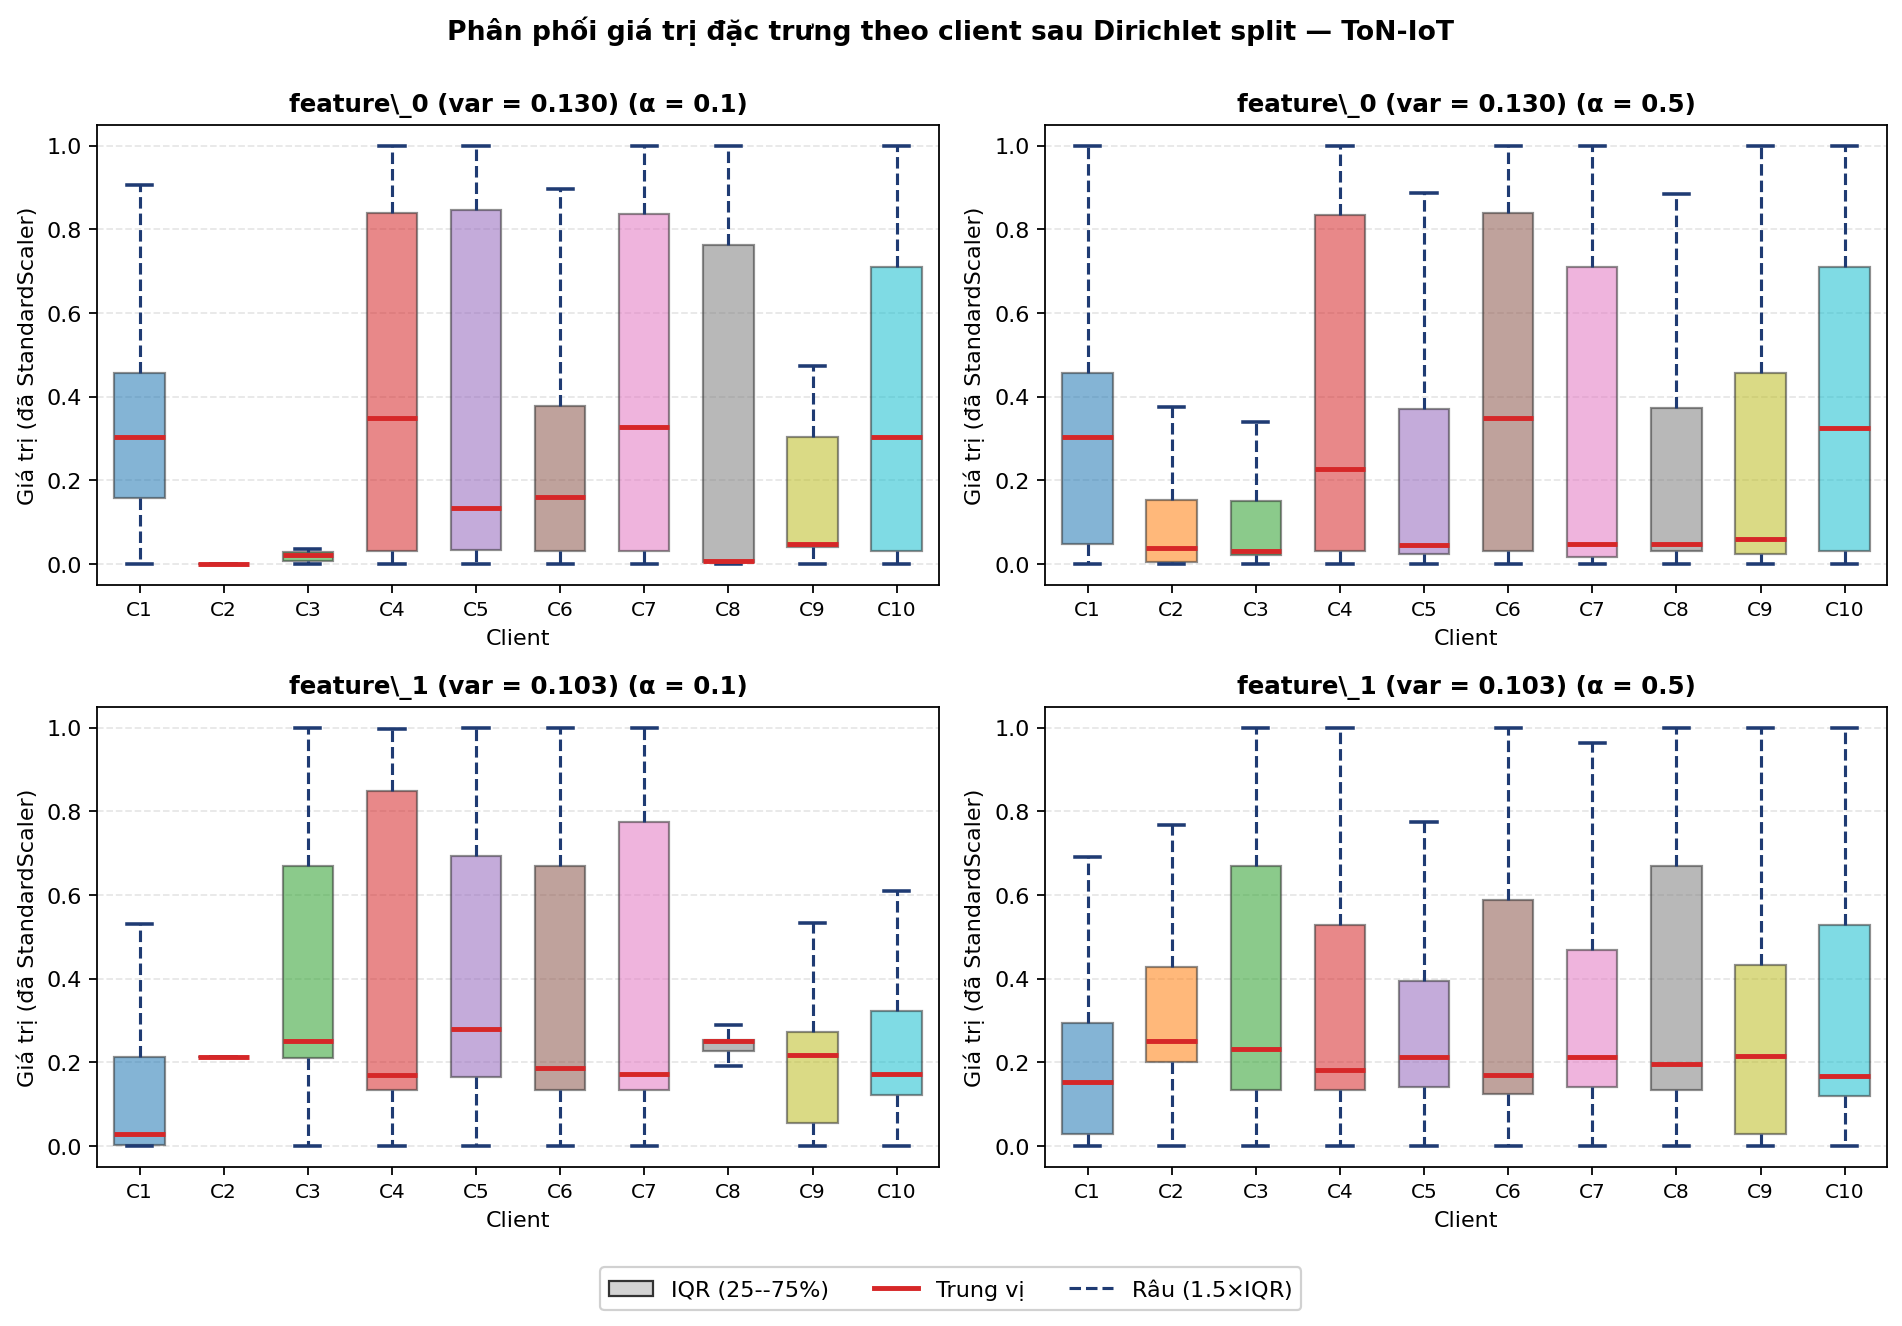
\includegraphics[width=0.95\linewidth]{Figures/fig_5_6_ton_iot_feature_skew_per_client.png}
    \caption{Phân phối giá trị đặc trưng theo client sau Dirichlet split -- ToN-IoT (\texttt{feature\_0} và \texttt{feature\_1}, hai cột có phương sai cao nhất sau StandardScaler; trái: $\alpha=0{,}1$, phải: $\alpha=0{,}5$)}
    \label{fig:ton_iot_feat_skew}
\end{figure}

Tóm lại, phân tích EDA cho thấy bốn đặc điểm quan trọng ảnh hưởng đến thực nghiệm: (1) cả hai dataset có mất cân bằng lớp nghiêm trọng, đòi hỏi Weighted Cross-Entropy Loss; (2) phân phối đặc trưng có nhiều outlier và nhiều bậc giá trị, ảnh hưởng đến chất lượng sinh dữ liệu của TabDDPM; (3) khi phân chia Dirichlet với $\alpha=0{,}1$, label skew trở nên cực đoan; (4) đồng thời feature skew cũng xuất hiện rõ rệt giữa các client. Hai dạng skew sau là nguyên nhân chính khiến các phương pháp phòng thủ thụ động nhầm client lành tính thành độc hại (Gap~2).

\section{Kịch bản A: Đánh giá hiệu năng phòng thủ}
Kịch bản A đánh giá hiệu năng phòng thủ của DT-Guard trên \textbf{hai bộ dữ liệu} (CIC-IoT-2023 và ToN-IoT) với \textbf{bốn mức tỉ lệ client độc hại} (10\%, 20\%, 40\%, 50\%), tổng cộng 5 tấn công $\times$ 4 tỉ lệ $\times$ 2 dataset = 40 kịch bản.

\subsection{Kết quả trên CIC-IoT-2023}
CIC-IoT-2023 có 39 đặc trưng và 34 lớp phân loại, được coi là kịch bản khó nhất trong hai dataset. Phần này phân tích kết quả qua hai hình minh chứng chính: \textbf{Hình 5.7} cho cặp Accuracy + Detection Rate và \textbf{Hình 5.8} cho heatmap FPR

\begin{figure}[H]
    \centering
    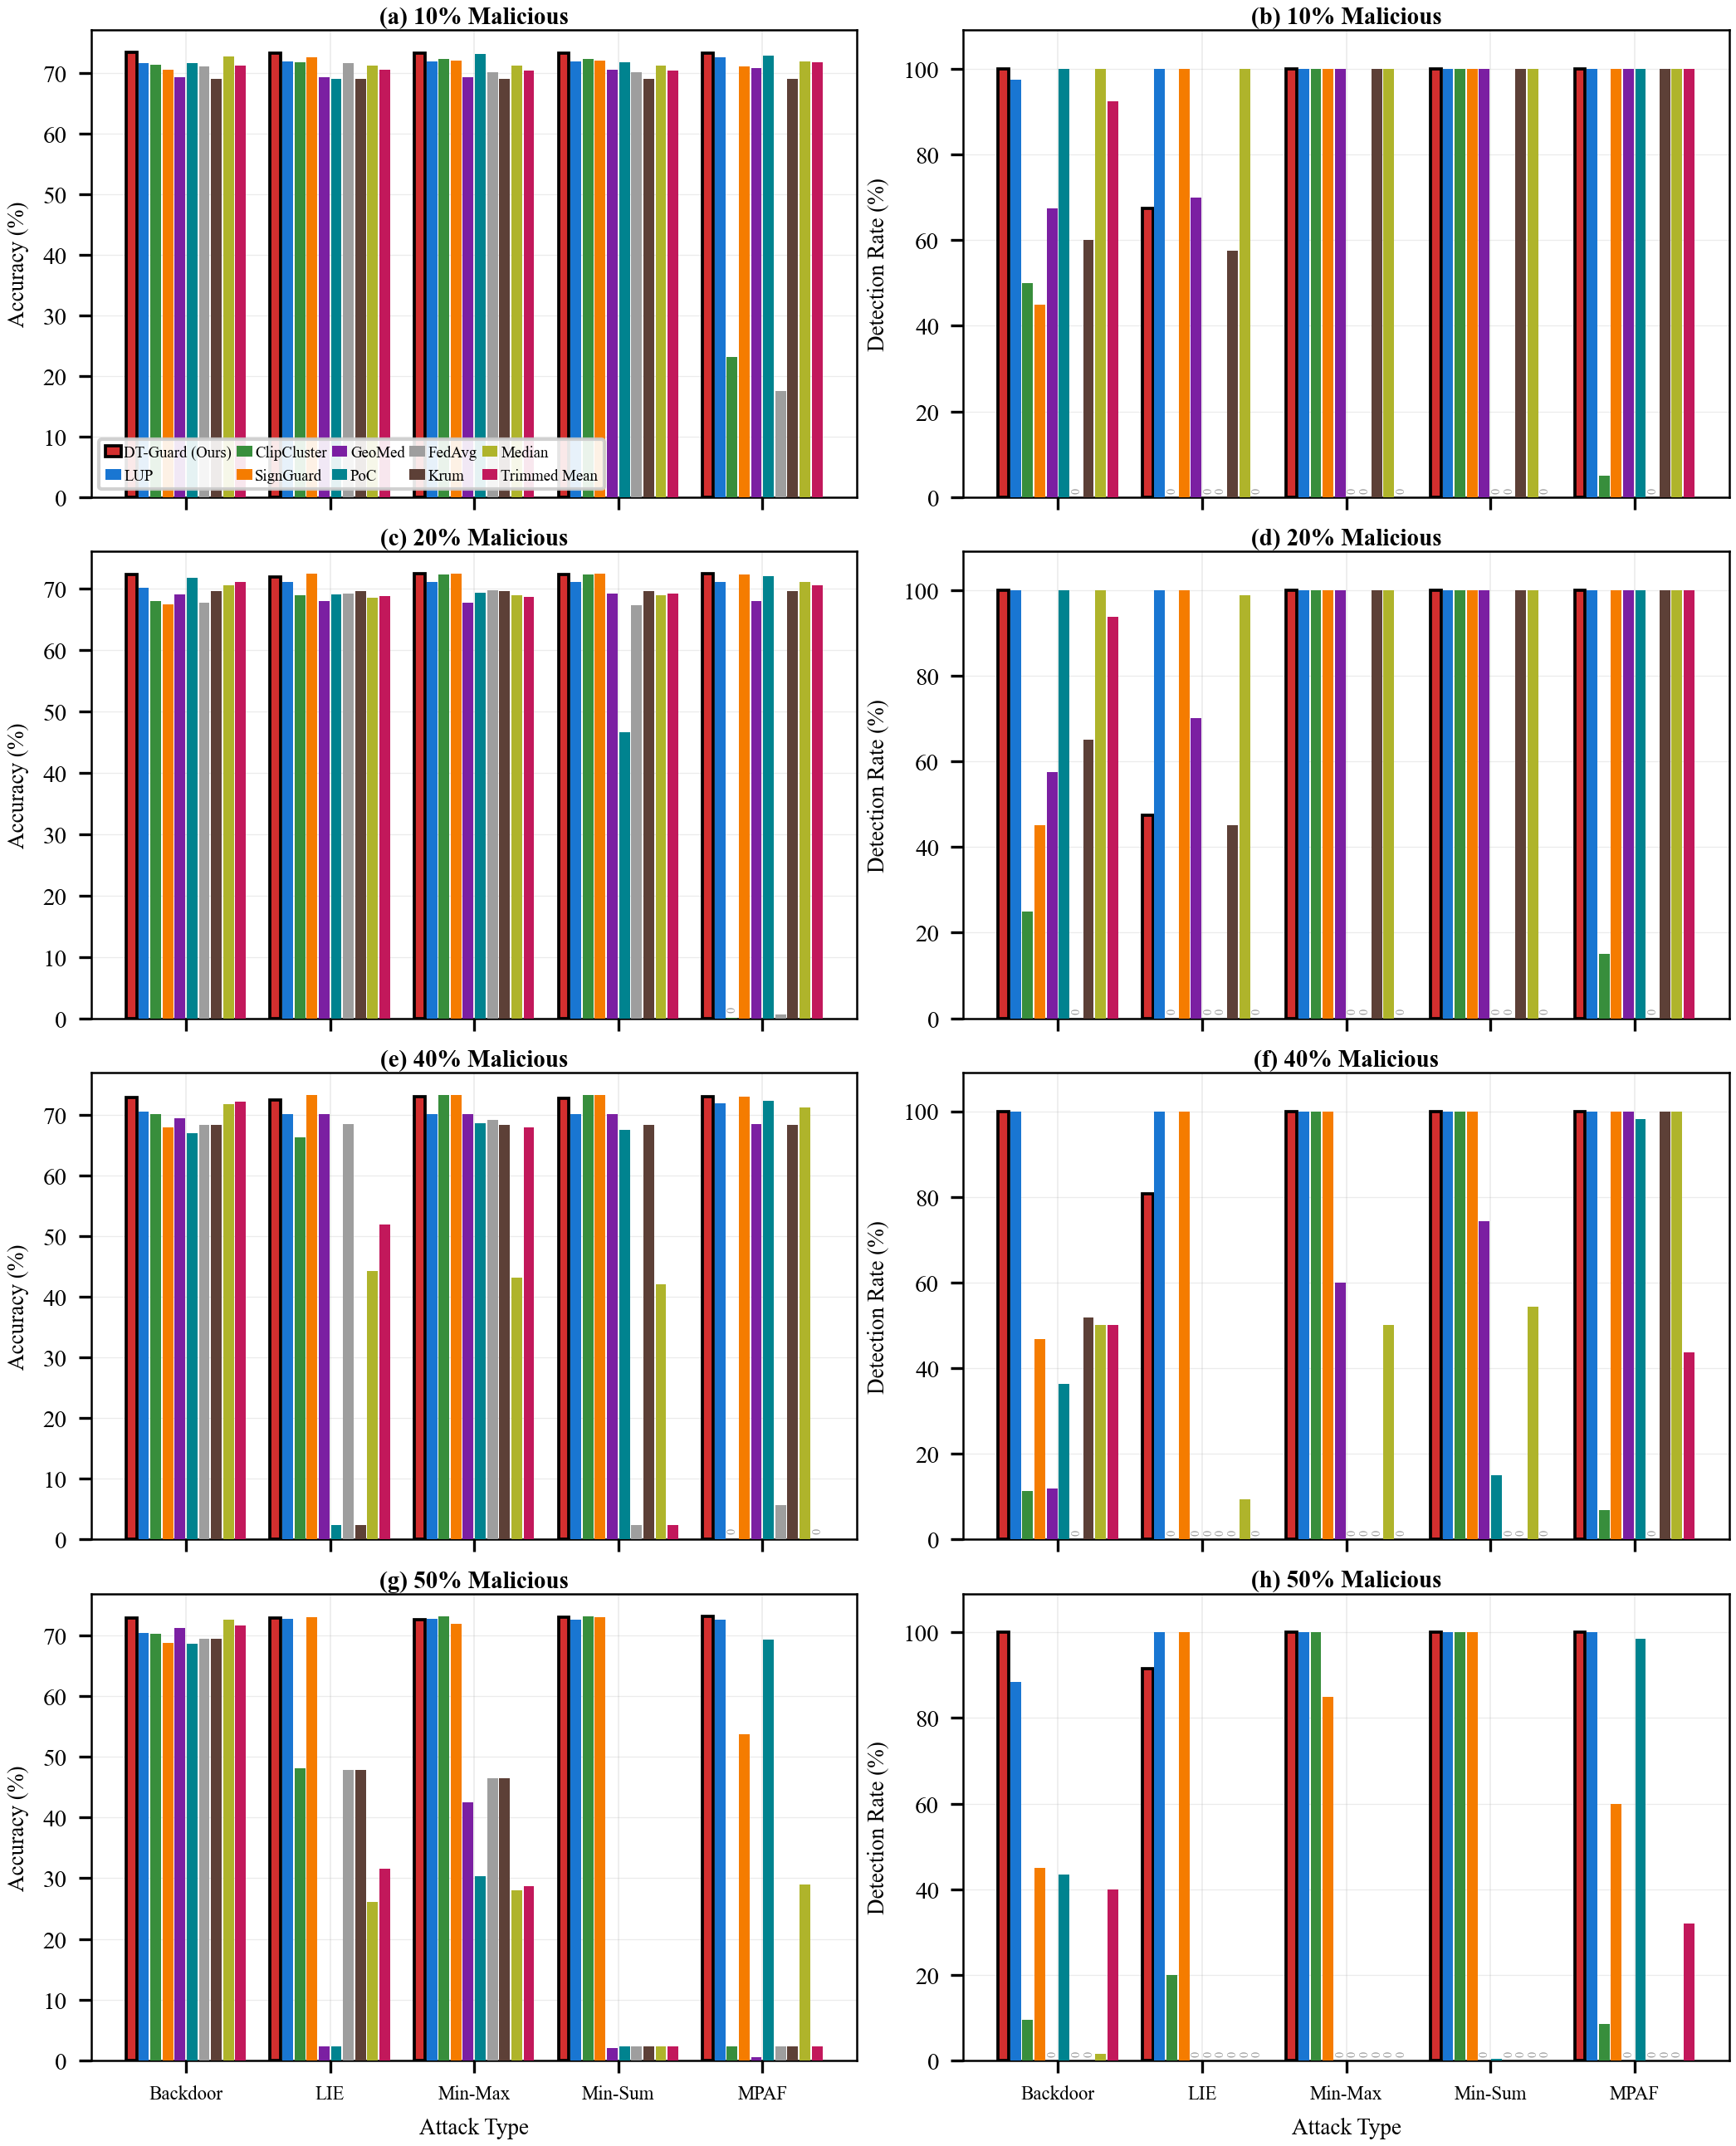
\includegraphics[width=0.85\linewidth]{Figures/fig_5_7_accuracy_dr_cic_iot_2023.png}
    \caption{Accuracy và Detection Rate trên CIC-IoT-2023 theo 4 mức tỉ lệ malicious}
\end{figure}

\textbf{Mỗi cặp panel ghép Accuracy của 10 phương pháp phòng thủ với Detection Rate tương ứng của DT-Guard trên 5 tấn công.}

\textbf{1)} DT-Guard giữ Accuracy ổn định bất chấp tỉ lệ tấn công. Bốn cột Accuracy của DT-Guard trong Hình 5.7 gần như cùng độ cao: trung bình 5 tấn công lần lượt là 73,26\% (10\%), 72,32\% (20\%), 72,74\% (40\%) và 72,84\% (50\%), biên độ dao động chưa đầy 1 điểm phần trăm. Khoảng {[}min, max{]} trên từng mức cũng rất hẹp: {[}73,19; 73,34{]}, {[}71,91; 72,49{]}, {[}72,40; 72,92{]} và {[}72,54; 73,09{]}. Điều này khẳng định pipeline kiểm chứng hành vi loại bỏ thành công bản cập nhật độc hại trước khi tổng hợp, mô hình toàn cục không bị "kéo lệch" dù tỉ lệ malicious tăng từ 10\% lên 50\%.

\textbf{2)} Detection Rate tăng dần khi tỉ lệ malicious tăng. Quan sát panel Detection Rate ở Hình 5.7, thanh DR trung bình của DT-Guard đi lên theo ratio: 93,5\% $\rightarrow$ 89,5\% $\rightarrow$ 96,1\% $\rightarrow$ 98,3\%. Tại mức 50\%, DT-Guard đạt 100\% trên Backdoor, Min-Max, Min-Sum, MPAF và 91,5\% trên LIE. Xu hướng tăng được giải thích như sau: khi nhiều attacker hơn, ảnh hưởng tập thể của các bản cập nhật độc hại trên không gian đặc trưng 39 chiều rõ rệt hơn, tạo sự phân biệt sắc nét hơn giữa hành vi suy luận lành tính và đầu độc trên challenge data. Riêng tấn công LIE có DR thấp nhất (67,5\% $\rightarrow$ 47,5\% $\rightarrow$ 80,6\% $\rightarrow$ 91,5\%) do biên độ nhiễu rất nhỏ, khó phân biệt khi số attacker còn ít. Điểm "lõm" tại 20\% (DR trung bình 89,5\%) hoàn toàn do LIE ở 20\% chỉ đạt 47,5\% kéo xuống, bốn tấn công còn lại vẫn 100\%.

\textbf{3)} Các baseline thất bại theo cơ chế cấu trúc, ngay cả ở mức malicious thấp. Đọc các nhóm cột trong panel Accuracy của Hình 5.7 từ trái sang phải:

\begin{itemize}
\item
  Nhóm không phòng thủ (FedAvg): Accuracy trung bình giảm theo ratio: 60,05\% (10\%) $\rightarrow$ 54,93\% (20\%) $\rightarrow$ 42,78\% (40\%) $\rightarrow$ 33,66\% (50\%). MPAF làm sụp FedAvg ở mọi ratio (17,49\% / 0,56\% / 5,67\% / 2,33\%) vì các fake clients chiếm đa số trọng số khi đơn thuần lấy trung bình. Min-Sum cũng kéo FedAvg xuống còn 2,33\% ở 40--50\% malicious.
\item
  Nhóm thống kê cổ điển (Krum, Median, Trimmed Mean, GeoMed): Cả bốn phương pháp này sụp nặng ở 50\% malicious: trung bình lần lượt 33,66\% (Krum), 31,61\% (Median), 27,29\% (Trimmed Mean), 23,76\% (GeoMed). Đặc biệt:

  \begin{itemize}
  \item
    Krum thất bại trước LIE (47,84\%) và sụp hoàn toàn trên Min-Sum, MPAF (cùng 2,33\%) vì các bản cập nhật độc hại tinh vi nằm ở giữa phân phối nên Krum chọn trúng chính chúng.
  \item
    Median sụp dưới Min-Sum (2,33\%), LIE (26,05\%), Min-Max (28,08\%), khi \textgreater50\% client là độc hại theo từng chiều, trung vị bị ảnh hưởng trực tiếp.
  \item
    Trimmed Mean sụp dưới Min-Sum (2,33\%) và MPAF (2,33\%); cắt outlier theo L2 norm không có tác dụng khi attack nằm trong phân phối lành tính.
  \item
    GeoMed sụp dưới LIE (2,33\%), Min-Sum (2,12\%), MPAF (0,60\%), geometric median bị kéo về cụm độc hại khi tỷ lệ tấn công lớn.
  \end{itemize}
\item
  Nhóm phân tích nâng cao (SignGuard, ClipCluster, LUP, PoC): Ba phương pháp đầu duy trì accuracy khá hơn nhưng vẫn có lỗ hổng đặc trưng:

  \begin{itemize}
  \item
    SignGuard sụp dưới MPAF (53,68\% ở 50\%) vì các fake clients có hướng dấu gradient đồng nhất, lọt qua bộ lọc dấu.
  \item
    ClipCluster sụp dưới MPAF ở mọi ratio (23,13\% $\rightarrow$ 0,05\% $\rightarrow$ 0,05\% $\rightarrow$ 2,33\%) vì các fake clients tạo cụm đông nhất, ClipCluster chọn nhầm cụm độc hại.
  \item
    LUP giữ accuracy cao nhất nhóm baseline (72,16\% trung bình ở 50\% malicious) nhưng phải đánh đổi bằng FPR rất cao (xem phần Phân tích False Positive Rate bên dưới).
  \item
    PoC sụp dưới LIE và Min-Sum ở 40--50\% (cùng 2,33\%) vì MMD đo khoảng cách tham số không phân biệt được Non-IID tự nhiên với đầu độc tinh vi.
  \end{itemize}
\end{itemize}

\begin{figure}[H]
    \centering
    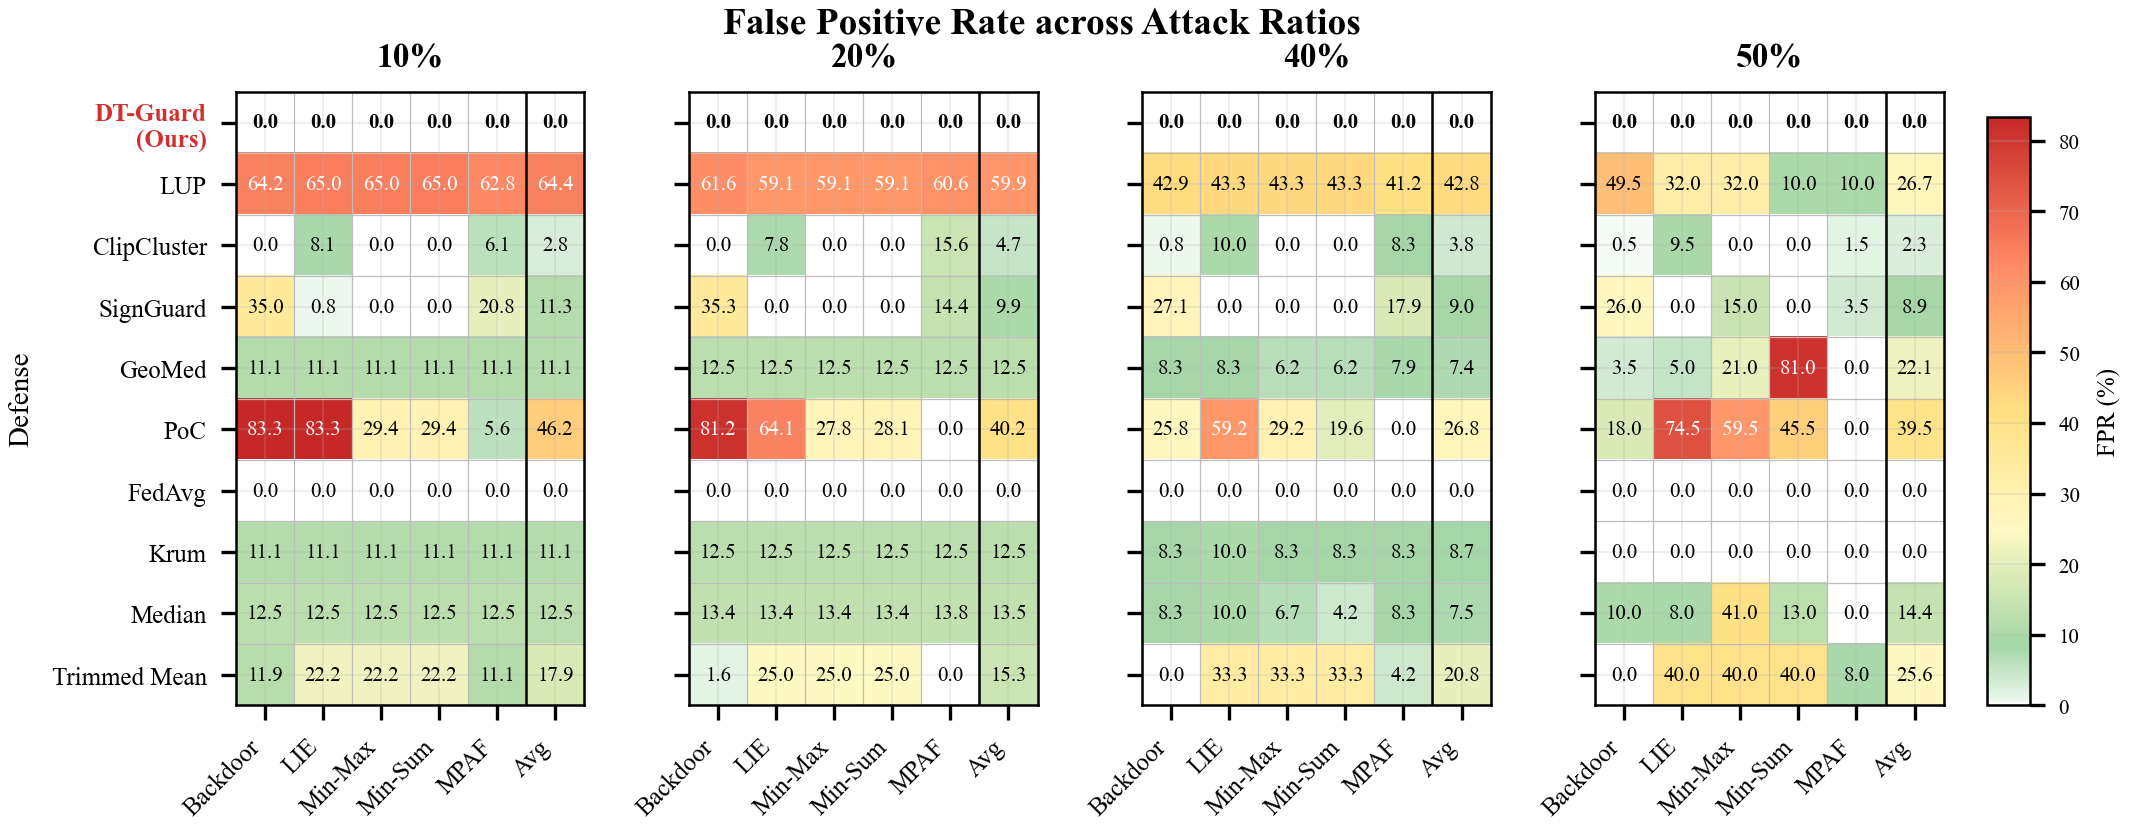
\includegraphics[width=0.85\linewidth]{Figures/fig_5_8_fpr_cic_iot_2023.png}
    \caption{Heatmap False Positive Rate (FPR) trên CIC-IoT-2023 theo 4 mức tỉ lệ malicious}
\end{figure}

\textbf{Mỗi ô là tỷ lệ client lành tính bị loại nhầm ở một cặp (defense, attack); ô càng đậm đỏ càng nhiều client bị loại oan.}

\textbf{Phân tích False Positive Rate (Hình 5.8)}

\textbf{1)} DT-Guard duy trì hàng FPR = 0\% xuyên suốt 20 ô (5 tấn công $\times$ 4 ratio). Hàng DT-Guard trong Hình 5.8 hoàn toàn trắng, không một client lành tính nào bị loại nhầm trong toàn bộ thực nghiệm trên CIC-IoT-2023. Đây là minh chứng trực tiếp cho luận điểm "kiểm chứng hành vi chủ động" của DT-Guard: bằng cách đo F1 trên challenge data thay vì so khoảng cách tham số, các client Non-IID lành tính vẫn vượt qua được Trust-Gate.

\textbf{2)} Hàng LUP có FPR cao bất thường, minh chứng cho Gap 2 (Non-IID confusion). LUP có FPR trung bình 64,39\% (10\%) $\rightarrow$ 59,87\% (20\%) $\rightarrow$ 42,83\% (40\%) $\rightarrow$ 26,70\% (50\%); riêng cell (LUP, Backdoor ở mức 10\%) đạt 65,00\%. Nghĩa là hơn nửa client lành tính bị MAD và hierarchical clustering của LUP đánh nhầm là outlier trong phần lớn kịch bản. Đây chính là điểm yếu cốt lõi của các phương pháp phân tích tham số thụ động khi gặp dữ liệu Non-IID nghiêm trọng.

\textbf{3)} Hàng PoC cũng có FPR rất cao (46,22\% $\rightarrow$ 40,25\% $\rightarrow$ 26,75\% $\rightarrow$ 39,50\% trung bình; đỉnh 83,33\% ở 10\% malicious). MMD đo khoảng cách phân phối tham số gặp đúng vấn đề như LUP.

\textbf{4)} Các baseline thống kê có FPR thấp hơn nhưng không "miễn phí". Krum, Median, GeoMed, Trimmed Mean có FPR trong khoảng 7--25\% trung bình, thấp hơn LUP/PoC nhưng vẫn loại nhầm 1--4 client lành tính mỗi vòng. Đáng chú ý: Krum ở mức 50\% có FPR = 0\% nhưng đó là vì nó \textbf{chọn duy nhất 1 client} mỗi vòng (không có khái niệm "loại nhầm"), đồng thời chính nó sụp accuracy còn 33,66\%. FedAvg cũng có FPR = 0\% chỉ vì không có cơ chế loại bỏ nào.

\textbf{Tổng kết cho CIC-IoT-2023}

Trên dataset khó nhất (39 đặc trưng, 34 lớp), DT-Guard cho thấy ba kết quả nhất quán: \textbf{(1)} Accuracy ổn định \textasciitilde73\% bất chấp tỉ lệ tấn công tăng 5 lần (10\% $\rightarrow$ 50\%); \textbf{(2)} Detection Rate trung bình tăng dần từ 89,5\% lên 98,3\% và đạt 100\% trên 4/5 tấn công ở mức malicious cao nhất; \textbf{(3)} FPR = 0\% trên toàn bộ 20 kịch bản. Trong khi đó, mọi baseline thuộc nhóm phân tích tham số thụ động đều bộc lộ lỗ hổng cấu trúc trước ít nhất một loại tấn công, hoặc phải đánh đổi accuracy bằng FPR cao (LUP, PoC), hoặc sụp accuracy nghiêm trọng (FedAvg, Krum, Median, Trimmed Mean, GeoMed) khi tỉ lệ malicious vượt 40\%.

\subsection{Kết quả trên ToN-IoT}
ToN-IoT có 10 đặc trưng và 10 lớp phân loại, không gian đặc trưng nhỏ hơn nhiều so với CIC-IoT-2023. Phần này áp dụng cùng bố cục phân tích: \textbf{Hình 5.9} cho cặp Accuracy + Detection Rate và \textbf{Hình 5.10} cho heatmap FPR

\begin{figure}[H]
    \centering
    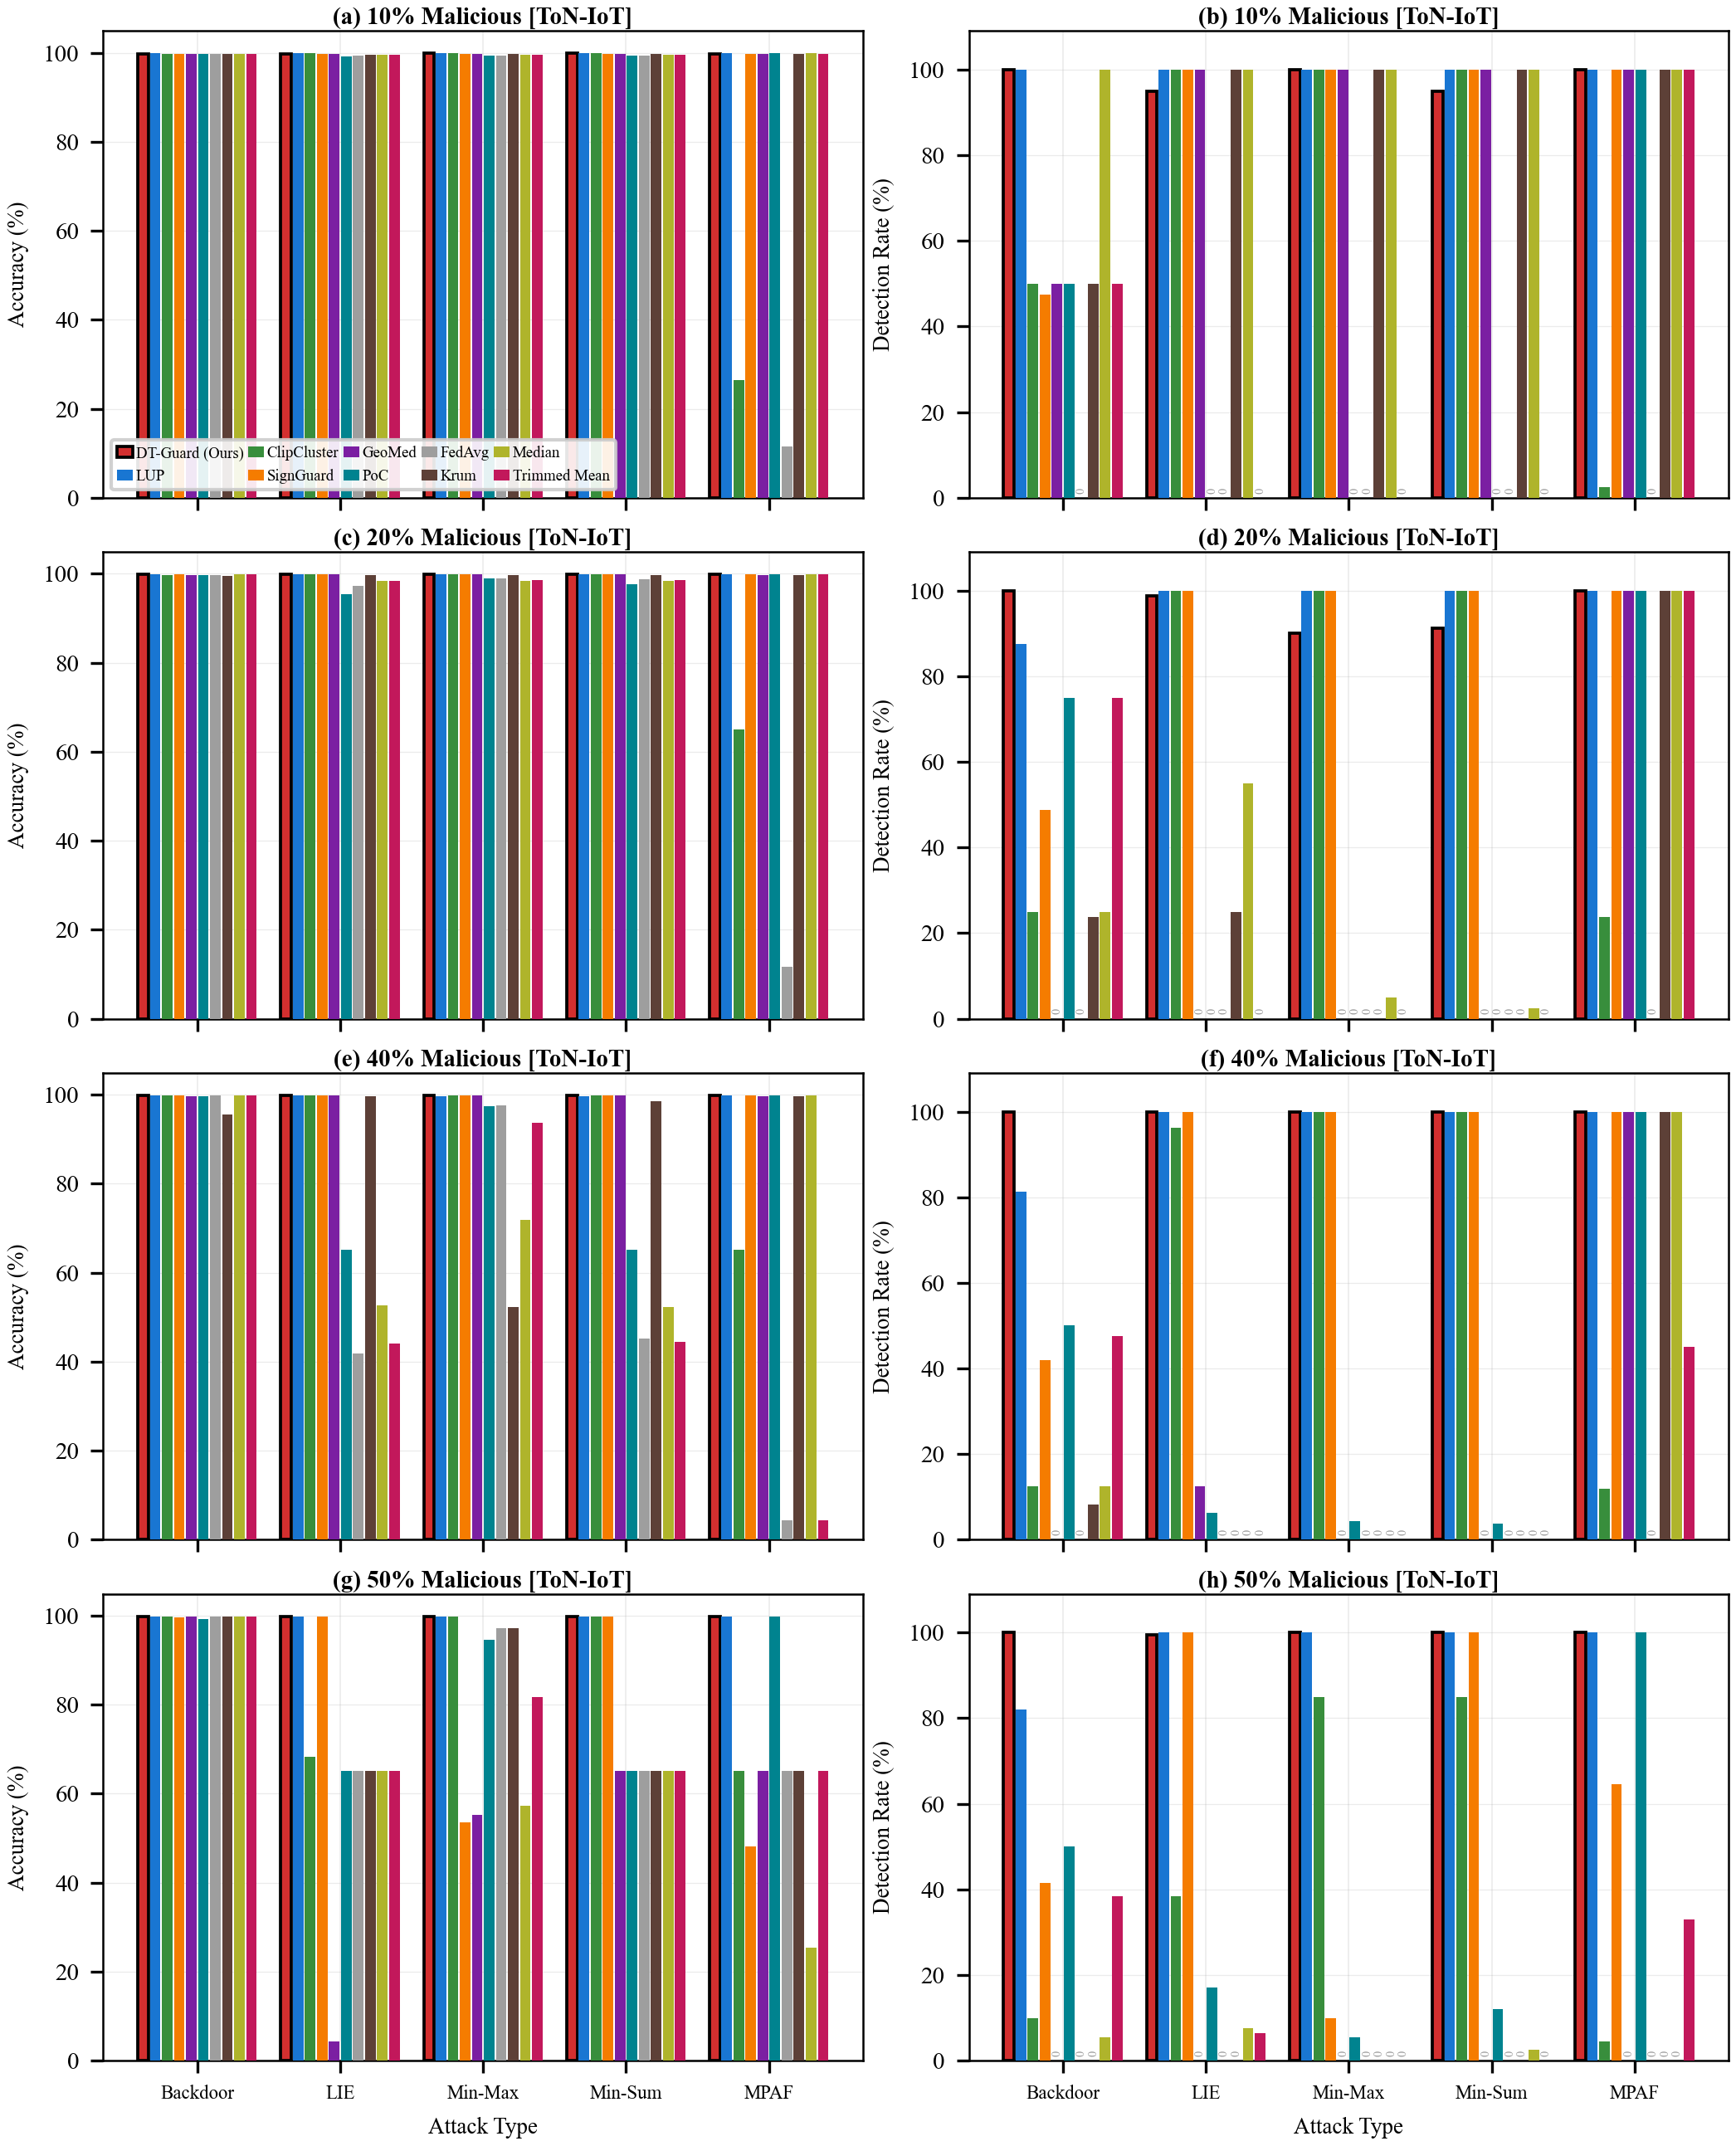
\includegraphics[width=0.85\linewidth]{Figures/fig_5_9_accuracy_dr_ton_iot.png}
    \caption{Accuracy và Detection Rate trên ToN-IoT theo 4 mức tỉ lệ malicious}
\end{figure}

\textbf{Mỗi cặp panel ghép Accuracy của 10 phương pháp phòng thủ với Detection Rate tương ứng của DT-Guard trên 5 tấn công.}

\textbf{Hiệu năng phát hiện xâm nhập (Hình 5.9), Accuracy và Detection Rate}

\textbf{1)} DT-Guard đạt accuracy gần như hoàn hảo và bất biến theo ratio. Bốn cột Accuracy của DT-Guard ở Hình 5.9 cùng cao đến mức gần trần: 99,81\% (10\%) $\rightarrow$ 99,80\% (20\%) $\rightarrow$ 99,84\% (40\%) $\rightarrow$ 99,83\% (50\%). Khoảng {[}min, max{]} cũng cực hẹp: {[}99,80; 99,83{]}, {[}99,78; 99,82{]}, {[}99,82; 99,86{]}, {[}99,81; 99,84{]}. So sánh với CIC-IoT-2023 (\textasciitilde73\%), accuracy cao hơn \textasciitilde27 điểm phần trăm phản ánh độ phức tạp bài toán: ToN-IoT chỉ có 10 lớp/10 đặc trưng nên kiến trúc MLP (256 $\rightarrow$ 128 $\rightarrow$ 64) đủ năng lực biểu diễn ranh giới phân loại; mất cân bằng lớp cũng nhẹ hơn (lớp lành tính chiếm \textasciitilde52\%).

\textbf{2)} Detection Rate đạt mức gần hoàn hảo ở ratio cao. Theo dõi panel Detection Rate ở Hình 5.9:

\begin{itemize}
\item
  \textbf{10\% malicious:} DT-Guard đạt 100\% trên Backdoor, Min-Max, MPAF; 95,0\% trên LIE và Min-Sum (DR trung bình 98,0\%).
\item
  \textbf{20\% malicious:} 100\% trên Backdoor và MPAF; 98,75\% trên LIE; 91,25\% trên Min-Sum; 90,0\% trên Min-Max (DR trung bình 96,0\%).
\item
  \textbf{40\% malicious:} \textbf{100\% trên cả 5 tấn công}, DT-Guard phát hiện toàn bộ attacker dù gần một nửa client là độc hại.
\item
  \textbf{50\% malicious:} 100\% trên Backdoor, Min-Max, Min-Sum, MPAF; 99,5\% trên LIE (DR trung bình 99,9\%).
\end{itemize}

So với CIC-IoT-2023 (LIE ở mức 50\% chỉ đạt 91,5\%), DR trên ToN-IoT vượt trội: ngay cả LIE, tấn công khó phát hiện nhất, cũng đạt 99,5\%. Nguyên nhân: trong không gian đặc trưng 10 chiều, mỗi chiều tham số có ảnh hưởng lớn hơn đến kết quả phân loại, do đó cùng một biên độ nhiễu của LIE tạo ra sai lệch hành vi rõ rệt hơn trên challenge data. Sự giảm nhẹ ở mức 20\% (DR Min-Max và Min-Sum giảm còn 90\% và 91,25\%) là do số attacker vẫn ít (4 client), chưa tạo được "đa số phá hoại" rõ rệt.

\textbf{3)} Các baseline thất bại theo đúng cơ chế đã quan sát trên CIC-IoT-2023. Đọc panel Accuracy ở Hình 5.9, ngay cả khi accuracy nền của ToN-IoT cao hơn nhiều, các baseline vẫn sụp đổ ở 50\% malicious:

\begin{itemize}
\item
  FedAvg sụp đồng loạt dưới LIE, Min-Sum và MPAF (cùng 65,07\%, tức về mức random guess) $\rightarrow$ trung bình 78,43\%.
\item
  Krum có pattern thất bại y hệt FedAvg (cùng 78,43\%, sụp dưới đúng 3 tấn công LIE/Min-Sum/MPAF cùng 65,07\%), minh chứng Krum không khác FedAvg khi tấn công lọt vào vùng trung tâm phân phối.
\item
  Median sụp dưới MPAF (25,48\%), LIE (65,07\%), Min-Max (57,34\%), Min-Sum (65,07\%) $\rightarrow$ trung bình 62,55\%.
\item
  Trimmed Mean sụp dưới LIE, Min-Sum, MPAF (cùng 65,07\%) $\rightarrow$ trung bình 75,36\%.
\item
  GeoMed sụp nặng nhất: LIE (4,34\%), Min-Max (55,14\%), Min-Sum (65,07\%), MPAF (65,07\%) $\rightarrow$ trung bình 57,86\% (thấp nhất nhóm).
\item
  ClipCluster sụp dưới LIE (68,19\%) và MPAF (65,07\%) $\rightarrow$ trung bình 86,53\%.
\item
  SignGuard sụp dưới Min-Max (53,53\%) và MPAF (48,17\%) $\rightarrow$ trung bình 80,18\%.
\item
  PoC sụp dưới LIE (65,07\%) và Min-Sum (65,07\%) $\rightarrow$ trung bình 84,75\%.
\item
  LUP là baseline duy nhất duy trì accuracy cao (99,84\% trung bình), nhưng phải đánh đổi bằng FPR cao (xem phần Phân tích False Positive Rate bên dưới).
\end{itemize}

\begin{figure}[H]
    \centering
    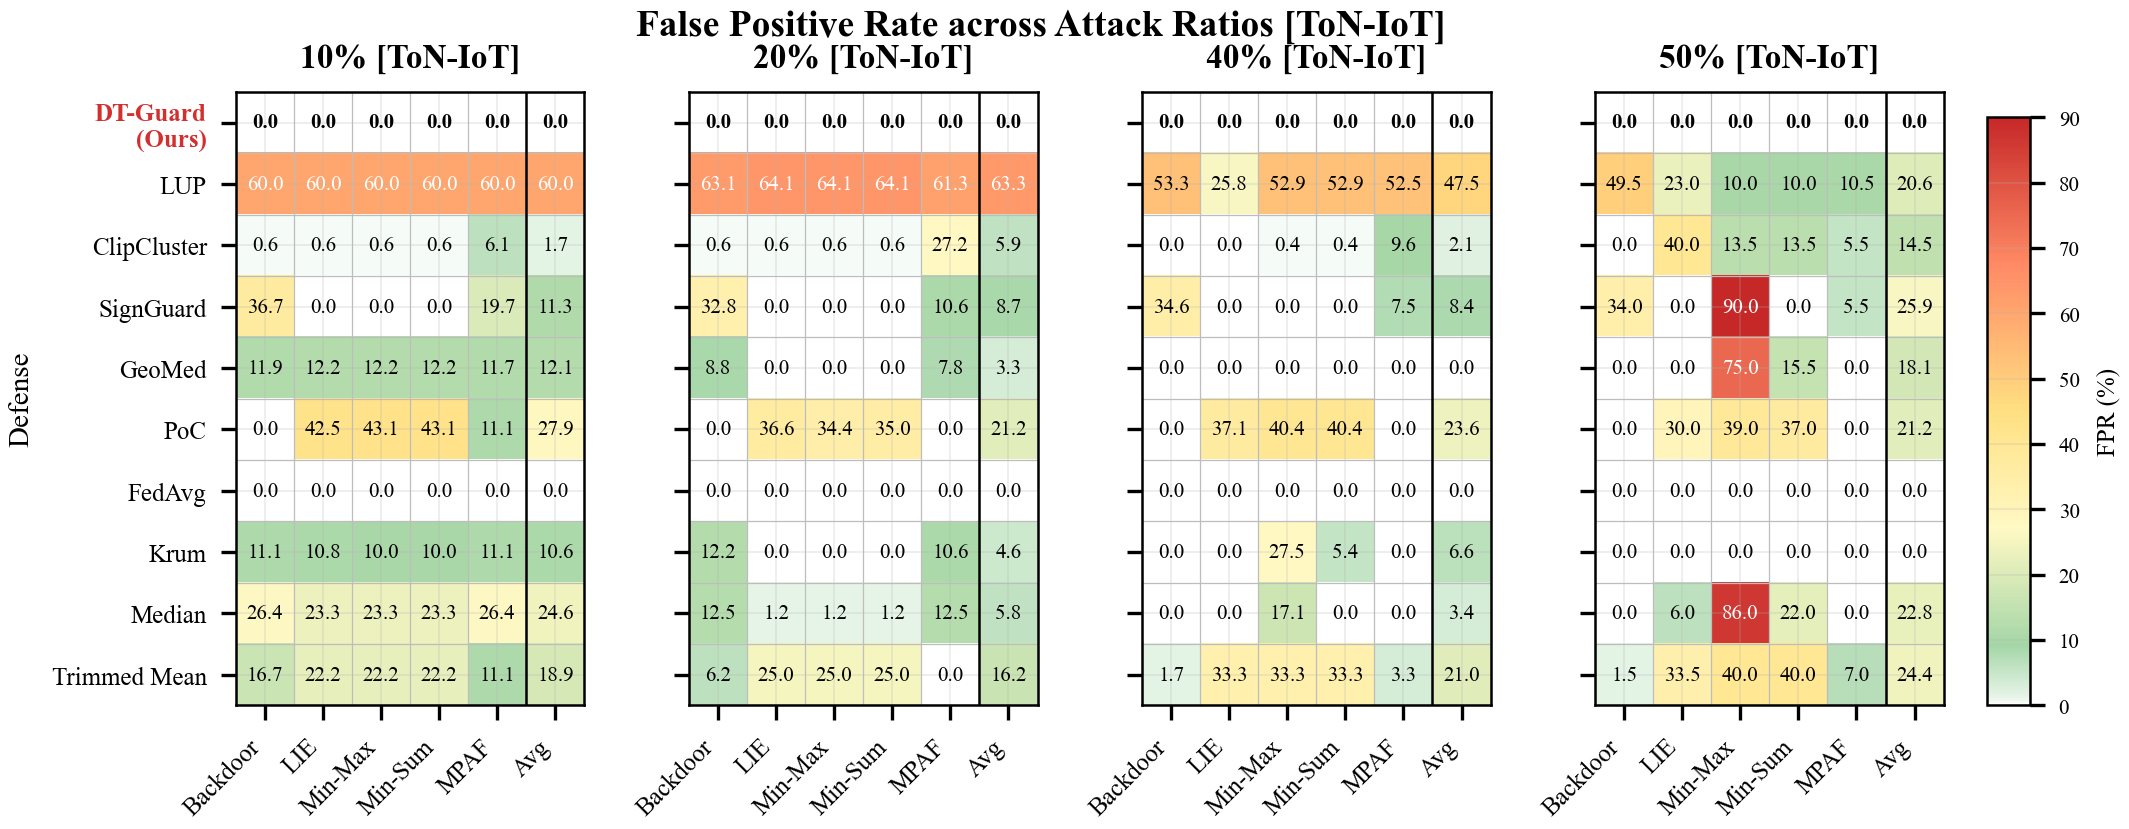
\includegraphics[width=0.85\linewidth]{Figures/fig_5_10_fpr_ton_iot.png}
    \caption{Heatmap False Positive Rate (FPR) trên ToN-IoT theo 4 mức tỉ lệ malicious}
\end{figure}

\textbf{Quan sát hàng DT-Guard hoàn toàn trắng so với hàng LUP, PoC, SignGuard có nhiều ô đỏ đậm.}

\textbf{Phân tích False Positive Rate (Hình 5.10)}

\textbf{1)} DT-Guard giữ FPR = 0\% xuyên suốt 20 ô. Hàng DT-Guard trong Hình 5.10 toàn trắng, kết quả nhất quán với CIC-IoT-2023 (Hình 5.8). Điều này xác nhận nguyên lý kiểm chứng hành vi không phụ thuộc kích thước không gian đặc trưng: client Non-IID lành tính ở cả 10 chiều và 39 chiều đều phân loại chính xác trên challenge data.

\textbf{2)} LUP có FPR rất cao ở mọi ratio. FPR trung bình của LUP: 60,00\% (10\%) $\rightarrow$ 63,31\% (20\%) $\rightarrow$ 47,50\% (40\%) $\rightarrow$ 20,60\% (50\%); đỉnh 64,06\% ở mức 20\% malicious. Mặc dù LUP giữ accuracy cao, mỗi vòng nó loại nhầm hơn nửa số client lành tính, minh chứng chính cho luận điểm "LUP thưởng cho các client trùng phân phối với mô hình toàn cục, đánh nhầm Non-IID lành tính là outlier."

\textbf{3)} Một số baseline có ô FPR rất đậm tại 50\% malicious. Đáng chú ý:

\begin{itemize}
\item
  SignGuard ở mức 50\%, Min-Max: FPR = 90,00\% (trung bình 25,90\%), chiều dấu gradient bị Min-Max thao túng đồng đều, SignGuard loại nhầm gần toàn bộ client lành tính.
\item
  Median ở mức 50\%, LIE: FPR = 86,00\% (trung bình 22,80\%), trung vị từng chiều bị "kéo" bởi cụm độc hại đồng nhất.
\item
  GeoMed ở mức 50\%, LIE: FPR = 75,00\% (trung bình 18,10\%).
\item
  PoC ổn định ở mức FPR cao 21--28\% trung bình qua mọi ratio.
\end{itemize}

\textbf{4)} Krum và FedAvg có FPR = 0\% nhưng đó không phải là điểm cộng. Krum chỉ chọn 1 client/vòng (không có khái niệm loại nhầm), FedAvg không có cơ chế lọc, cả hai đều phải trả giá bằng accuracy thấp như đã phân tích ở phần Hiệu năng phát hiện xâm nhập.

\textbf{Tổng kết cho ToN-IoT}

Trên dataset đơn giản hơn (10 đặc trưng, 10 lớp), DT-Guard cho ba kết quả mạnh hơn cả trên CIC-IoT-2023: \textbf{(1)} Accuracy $\approx$ 99,8\% bất biến qua 4 ratio; \textbf{(2)} Detection Rate đạt 100\% trên cả 5 tấn công ngay từ ratio 40\% và duy trì 99,9\% ở 50\%; \textbf{(3)} FPR = 0\% trên toàn bộ 20 kịch bản. Cùng các baseline cũng dễ phòng thủ hơn ở ratio thấp (\textasciitilde99\% accuracy ở 10--20\%) nhưng vẫn sụp đổ ở 50\% malicious theo đúng cơ chế thất bại đã quan sát trên CIC-IoT-2023, tái xác nhận tính cấu trúc (chứ không phải tham số) của lỗ hổng.

\subsection{So sánh chéo giữa hai dataset}
Việc đánh giá trên hai dataset khác biệt hoàn toàn, CIC-IoT-2023 (34 lớp, 39 đặc trưng, IoTAttackNet/MLP) và ToN-IoT (10 lớp, 10 đặc trưng, MLP), cho phép rút ra kết luận quan trọng về tính tổng quát hóa của cả phương pháp đề xuất lẫn các baseline.

\textbf{Sự nhất quán của DT-Guard trên cả hai dataset:} Cả CIC-IoT-2023 và ToN-IoT đều cho thấy ba đặc trưng ổn định: (1) accuracy duy trì ổn định qua mọi mức malicious; (2) Detection Rate cao và tăng dần khi tỉ lệ malicious tăng; (3) FPR = 0,0\% trên tất cả kịch bản. Nguyên lý kiểm chứng hành vi hoạt động hiệu quả bất kể kích thước không gian đặc trưng (39 vs. 10), số lớp phân loại (34 vs. 10), hay mức độ mất cân bằng lớp, vì pipeline đánh giá trực tiếp năng lực phân loại trên challenge data chứ không phụ thuộc vào đặc trưng cụ thể của dataset.

\textbf{Sự nhất quán trong cơ chế thất bại của baseline:} ClipCluster luôn sụp dưới MPAF, GeoMed luôn sụp dưới LIE, SignGuard luôn sụp dưới Min-Max và Min-Sum, bất kể dataset nào. Điều này chứng tỏ lỗ hổng của nhóm phương pháp chỉ phân tích đặc trưng tĩnh của tham số là \textbf{cấu trúc}, không phải do tham số tinh chỉnh kém, không phải do đặc thù dataset, mà do bản thân cách tiếp cận thụ động không thể phân biệt giữa tham số bình thường và tham số bị đầu độc tinh vi. Việc cùng một phương pháp thất bại trước cùng loại tấn công ở cả hai môi trường thử nghiệm cho thấy lỗ hổng là cố hữu trong thiết kế, không phụ thuộc ngữ cảnh.

\textbf{Điểm khác biệt đáng chú ý giữa hai dataset:} Trên ToN-IoT, DR đạt 100\% ở mọi tấn công ngay từ mức 40\% malicious, trong khi trên CIC-IoT-2023, cần đến 50\% malicious mới đạt 98,3\%. Accuracy trên ToN-IoT (99,83\%) cũng cao hơn đáng kể so với CIC-IoT-2023 (72,8\%). Sự khác biệt này phản ánh mức độ khó của bài toán phân loại chứ không phải hiệu năng của DT-Guard, ToN-IoT có 10 lớp và 10 đặc trưng nên mô hình phân loại chính xác hơn và các dấu hiệu đầu độc cũng dễ phát hiện hơn trong không gian nhỏ. Kết quả này cho thấy DT-Guard hiệu quả hơn trên các bài toán có không gian đặc trưng nhỏ, nhưng vẫn bảo vệ đầy đủ trên bài toán phức tạp hơn (CIC-IoT-2023) mà không có sự suy giảm nghiêm trọng nào.

DT-Guard khắc phục được lỗ hổng cấu trúc của các phương pháp thụ động nhờ đánh giá hành vi suy luận thực tế, nguyên lý này tổng quát, không phụ thuộc vào đặc trưng dataset hay kiến trúc mô hình IDS.

\subsection{Giải thích hiện tượng đặc biệt}
\textbf{Hiện tượng 1:} DR tăng khi tỉ lệ malicious tăng. Đây là một xu hướng thoạt nhìn có vẻ phản trực giác: càng nhiều client độc hại thì lại càng dễ phát hiện. Nguyên nhân nằm ở cơ chế tổng hợp FedAvg: khi tỉ lệ malicious tăng, tổng trọng số của các bản cập nhật độc hại trong mô hình toàn cục cũng tăng theo. Mô hình toàn cục bị nhiễu nhiều hơn, khiến mô hình cục bộ của client lành tính (không bị đầu độc) có hành vi phân loại ngày càng khác biệt so với mô hình toàn cục trên challenge data. Khoảng cách hành vi này tạo ra sự phân tách rõ nét hơn trong Trust-Score, client độc hại có F1 thấp trên challenge data trong khi client lành tính vẫn phân loại chính xác. Hơn nữa, khi số lượng attacker lớn hơn, pattern đầu độc cũng đồng nhất hơn (các attacker cùng thực hiện một chiến thuật), tạo ra cụm hành vi đặc trưng dễ nhận diện hơn so với khi chỉ có 1--2 attacker bị chìm giữa nhiều client lành tính.

Cụ thể, trên CIC-IoT-2023: DR trung bình tăng từ 93,5\% (10\%) $\rightarrow$ 89,5\% (20\%) $\rightarrow$ 96,1\% (40\%) $\rightarrow$ 98,3\% (50\%). Ngoại lệ nhỏ ở mức 20\% (89,5\% thấp hơn 93,5\% ở mức 10\%) là do ở tỉ lệ này, LIE attack chỉ đạt DR 47,5\%, mức thấp nhất kéo trung bình xuống. Ở 10\% malicious (2 client độc hại), LIE được phát hiện 67,5\% nhờ vào 2 attacker này tạo ra một sự khác biệt vừa đủ trong hành vi. Nhưng khi tăng lên 20\% (4 attacker), LIE vẫn thay đổi rất ít tham số và 4 attacker chưa đủ tạo ra pattern rõ ràng, nên DR giảm tạm thời. Khi vượt qua ngưỡng 40\% (8 attacker), ảnh hưởng tập thể đủ mạnh để pipeline nhận diện.

\textbf{Hiện tượng 2:} LIE là tấn công khó phát hiện nhất. Trên cả hai dataset, LIE luôn có DR thấp nhất trong 5 tấn công (67,5\% tại 10\% malicious trên CIC-IoT-2023, và cũng là tấn công cuối cùng đạt 100\% DR trên ToN-IoT). Nguyên nhân gốc rễ nằm ở chiến lược thiết kế của LIE: thay đổi tham số "vừa đủ" để nằm trong vùng phân phối thống kê bình thường, cụ thể, attacker cộng thêm một lượng z $\times$ $\sigma$ vào giá trị trung bình mỗi chiều, với z được điều chỉnh cẩn thận. Lượng thay đổi này rất nhỏ so với các tấn công khác như MPAF (nhân bản update $\times10)$ hay Backdoor (thay đổi chuyên biệt 2 lớp cuối), nên hành vi suy luận của mô hình bị đầu độc cũng chỉ sai lệch nhẹ trên challenge data. Pipeline 4 lớp vẫn phát hiện được nhờ đánh giá trực tiếp F1 trên challenge data thay vì chỉ nhìn khoảng cách tham số, nhưng cần nhiều "bằng chứng" hơn (nhiều mẫu challenge, tỉ lệ malicious cao hơn) để phân biệt giữa sai lệch nhỏ ngẫu nhiên và sai lệch do đầu độc.

Tuy nhiên, kết quả quan trọng là: ngay cả với LIE, tấn công khó nhất, DT-Guard vẫn đạt DR 91,5\% tại 50\% malicious trên CIC-IoT-2023 và 99,5\% trên ToN-IoT. Điều này cho thấy pipeline kiểm chứng hành vi có khả năng chịu đựng ngay cả với các tấn công được thiết kế tinh vi nhất, miễn là tỉ lệ độc hại đủ cao để tạo ra dấu hiệu nhận diện.

\textbf{Hiện tượng 3:} Accuracy gần như không đổi khi tỉ lệ malicious tăng. Trên CIC-IoT-2023, accuracy dao động trong khoảng hẹp 72,3\%--73,3\% qua cả 4 mức tỉ lệ malicious; trên ToN-IoT, accuracy ổn định ở 99,80\%--99,84\%. Hiện tượng này cho thấy DT-Guard loại bỏ hiệu quả các bản cập nhật độc hại trước khi tổng hợp, chỉ các client vượt qua Trust Gate mới tham gia vào mô hình toàn cục. Kết quả là mô hình toàn cục không bị suy giảm dù tỉ lệ tấn công tăng từ 10\% lên 50\%. Tuy nhiên, accuracy không tăng khi tỉ lệ malicious giảm (từ 50\% xuống 10\%) vì accuracy chủ yếu bị giới hạn bởi khả năng phân loại của mô hình IDS trên bài toán 34 lớp (CIC-IoT-2023) chứ không phải bởi tấn công, tức là mô hình đã đạt "trần" hiệu năng cho kiến trúc MLP trên bài toán này.

\section{Kịch bản B: Đánh giá bộ sinh dữ liệu thách thức}

\subsection{Kết quả A/B Testing}
Năm mô hình sinh được đánh giá trên CIC-IoT-2023 qua bốn nhóm tiêu chí. Bảng 5.1 tổng hợp kết quả chi tiết, giá trị tốt nhất mỗi tiêu chí được in đậm.

\begin{longtable}[]{@{}
  >{\raggedright\arraybackslash}p{(\linewidth - 10\tabcolsep) * \real{0.1821}}
  >{\raggedright\arraybackslash}p{(\linewidth - 10\tabcolsep) * \real{0.1730}}
  >{\raggedright\arraybackslash}p{(\linewidth - 10\tabcolsep) * \real{0.1352}}
  >{\raggedright\arraybackslash}p{(\linewidth - 10\tabcolsep) * \real{0.2258}}
  >{\raggedright\arraybackslash}p{(\linewidth - 10\tabcolsep) * \real{0.1427}}
  >{\raggedright\arraybackslash}p{(\linewidth - 10\tabcolsep) * \real{0.1412}}@{}}
\caption{So sánh chi tiết năm mô hình sinh dữ liệu trên CIC-IoT-2023} \\
\toprule\noalign{}
\begin{minipage}[b]{\linewidth}\centering
\textbf{Tiêu chí}
\end{minipage} & \begin{minipage}[b]{\linewidth}\centering
\textbf{TabDDPM}
\end{minipage} & \begin{minipage}[b]{\linewidth}\centering
\textbf{TabSyn}
\end{minipage} & \begin{minipage}[b]{\linewidth}\centering
\textbf{ForestDiffusion}
\end{minipage} & \begin{minipage}[b]{\linewidth}\centering
\textbf{CTGAN}
\end{minipage} & \begin{minipage}[b]{\linewidth}\centering
\textbf{WGAN-GP}
\end{minipage} \\
\midrule\noalign{}
\endfirsthead
%
\multicolumn{6}{c}{{\textit{(tiếp) Bảng 5.2}}} \\
\toprule\noalign{}
\begin{minipage}[b]{\linewidth}\centering
\textbf{Tiêu chí}
\end{minipage} & \begin{minipage}[b]{\linewidth}\centering
\textbf{TabDDPM}
\end{minipage} & \begin{minipage}[b]{\linewidth}\centering
\textbf{TabSyn}
\end{minipage} & \begin{minipage}[b]{\linewidth}\centering
\textbf{ForestDiffusion}
\end{minipage} & \begin{minipage}[b]{\linewidth}\centering
\textbf{CTGAN}
\end{minipage} & \begin{minipage}[b]{\linewidth}\centering
\textbf{WGAN-GP}
\end{minipage} \\
\midrule\noalign{}
\endhead
\bottomrule\noalign{}
\endlastfoot
\textbf{Fidelity} & & & & & \\
TSTR (\%) & \textbf{71,4} & 66,4 & 55,1 & 55,3 & 66,0 \\
TRTR baseline (\%) & 69,1 & 69,1 & 69,1 & 69,1 & 69,1 \\
Wasserstein Dist. & \textbf{0,061} & 0,085 & 16,667 & 0,213 & 0,323 \\
Jensen-Shannon Dist. & 0,039 & \textbf{0,025} & 0,044 & 0,016 & 0,060 \\
\textbf{Coverage \& Diversity} & & & & & \\
Recall & 0,982 & 0,449 & \textbf{1,000} & 0,915 & 0,277 \\
Precision & 0,223 & 0,258 & 0,196 & \textbf{0,685} & 0,051 \\
Coverage & 0,075 & 0,061 & 0,002 & \textbf{0,347} & 0,002 \\
DCR ($\downarrow$) & 0,0053 & 0,0069 & 0,1253 & \textbf{0,0048} & 0,0174 \\
\textbf{Conditional Control} & & & & & \\
Label Accuracy (\%) & 61,2 & \textbf{70,0} & 0,9 & 60,5 & 51,9 \\
\textbf{Efficiency} & & & & & \\
Training Time (s) & 200 & \textbf{140} & 856 & 1606 & 6 \\
Peak RAM (MB) & 25 & 25 & 82 & \textbf{177} & 9 \\
\textbf{Ứng dụng DT-Guard} & & & & & \\
DT Separation & 0,538 & \textbf{0,708} & $-0,028$ & 0,500 & 0,496 \\
\end{longtable}

\textbf{Fidelity (Độ trung thực):} TabDDPM đạt TSTR 71,4\%, cao nhất và vượt cả baseline TRTR 69,1\% (huấn luyện và kiểm tra đều trên dữ liệu thật), cho thấy dữ liệu sinh không chỉ phản ánh phân phối thực mà còn hỗ trợ học transfer hiệu quả. TabSyn (66,4\%) và WGAN-GP (66,0\%) thuộc nhóm thứ hai, thấp hơn TabDDPM khoảng 5 điểm phần trăm. ForestDiffusion (55,1\%) và CTGAN (55,3\%) có TSTR thấp nhất, thấp hơn TabDDPM hơn 16 điểm phần trăm. Về Wasserstein Distance, TabDDPM đạt 0,061 (thấp nhất), TabSyn 0,085, CTGAN 0,213, WGAN-GP 0,323, trong khi ForestDiffusion lên tới 16,667, cho thấy TabDDPM sinh phân phối sát thực nhất. Sự chênh lệch lớn giữa TabDDPM và ForestDiffusion ở Wasserstein Distance phản ánh vấn đề mô hình cây sinh dữ liệu ở không gian gốc thay vì học phân phối liên tục, tạo ra khoảng cách lớn về phân phối biên. Nguyên nhân nhóm Diffusion vượt trội: tối ưu hóa trực tiếp quá trình khử nhiễu theo từng bước với mục tiêu rõ ràng (tối thiểu hóa sai số nhiễu), trong khi GAN tối ưu hóa gián tiếp qua zero-sum game giữa Generator và Discriminator, dễ rơi vào trạng thái bất ổn định (mode collapse) hoặc học được phân phối bị lệch.

\textbf{Coverage \& Diversity (Bao phủ và đa dạng):} TabDDPM đạt Recall 0,982, gần bao phủ toàn bộ các vùng của phân phối thực, chỉ bỏ sót 1,8\%. ForestDiffusion đạt Recall hoàn hảo 1,000 nhưng Precision chỉ 0,196, bao phủ rộng nhưng sinh nhiều mẫu không đại diện (nhiễu). Ngược lại, CTGAN đạt Precision cao nhất 0,685 nhưng Recall 0,915, mẫu sinh chất lượng nhưng bỏ sót 8,5\% phân phối thực, hiện tượng mode collapse đặc trưng của GAN. WGAN-GP có Recall thấp nhất 0,277, bỏ sót hơn 72\% phân phối thực, cho thấy mode collapse nghiêm trọng. Về DCR (Distance to Closest Record), cả TabDDPM (0,0053) và CTGAN (0,0048) đều cho thấy mẫu sinh gần dữ liệu huấn luyện nhưng không trùng lặp trực tiếp. ForestDiffusion có DCR 0,1253, mẫu sinh xa dữ liệu gốc, phản ánh khả năng khử nhiễu hạn chế của mô hình cây trong không gian nhiều chiều.

\textbf{Conditional Control (Kiểm soát điều kiện):} Đây là tiêu chí quan trọng nhất cho DT-Guard vì bộ sinh cần tạo challenge data cân bằng nhãn, mỗi lớp tấn công cần số mẫu tương đương. TabSyn đạt Label Accuracy cao nhất 70,0\%, tiếp theo là TabDDPM 61,2\% và CTGAN 60,5\%. WGAN-GP chỉ đạt 51,9\%, gần mức ngẫu nhiên cho bài toán đa lớp, cho thấy conditional generation gần như không hoạt động. ForestDiffusion đạt thấp nhất 0,9\%, XGBoost không có cơ chế điều kiện tự nhiên nên gần như không kiểm soát được nhãn sinh. TabDDPM đạt 61,2\%, kết quả chấp nhận được vì kết hợp với Recall 0,982 đảm bảo bao phủ đa dạng; độ chính xác trung bình được bù đắp bởi việc sinh nhiều mẫu rồi lấy cân bằng nhãn trong bước sampling.

\textbf{Efficiency (Hiệu quả):} WGAN-GP có thời gian huấn luyện nhanh nhất (6 giây) nhưng chất lượng sinh kém nhất ở mọi tiêu chí khác. Trong các mô hình chất lượng cao, TabDDPM (200 giây) nhanh gấp 8 lần CTGAN (1606 giây) và nhanh gấp 4 lần ForestDiffusion (856 giây). TabSyn đạt 140 giây nhưng TSTR và Recall thấp hơn TabDDPM. TabDDPM tiêu thụ peak RAM 25 MB, tiết kiệm gấp 7 lần CTGAN (177 MB) và gấp 3 lần ForestDiffusion (82 MB).

\textbf{Tổng hợp:} TabDDPM đạt composite score cao nhất (7,3/10) nhờ sự cân bằng tốt giữa bốn tiêu chí: TSTR cao nhất, Wasserstein Distance thấp nhất, Recall gần 1,0, và training time chỉ 200 giây. Kết quả quan trọng nhất ở hàng "DT Separation" cho thấy TabDDPM tạo ra challenge data giúp DT-Guard phân biệt rõ nhất giữa client lành tính và độc hại (0,538). ForestDiffusion có DT Separation âm ($-$0,028), dữ liệu sinh kém chất lượng khiến pipeline đánh giá sai. Kết quả này cho thấy mô hình Diffusion, khi được thiết kế chuyên biệt cho dữ liệu bảng như TabDDPM, vượt trội hơn so với cả GAN và các phương pháp lai (VAE + diffusion) trong bối cảnh sinh dữ liệu thách thức cho hệ thống FL-IDS.

\begin{figure}[H]
    \centering
    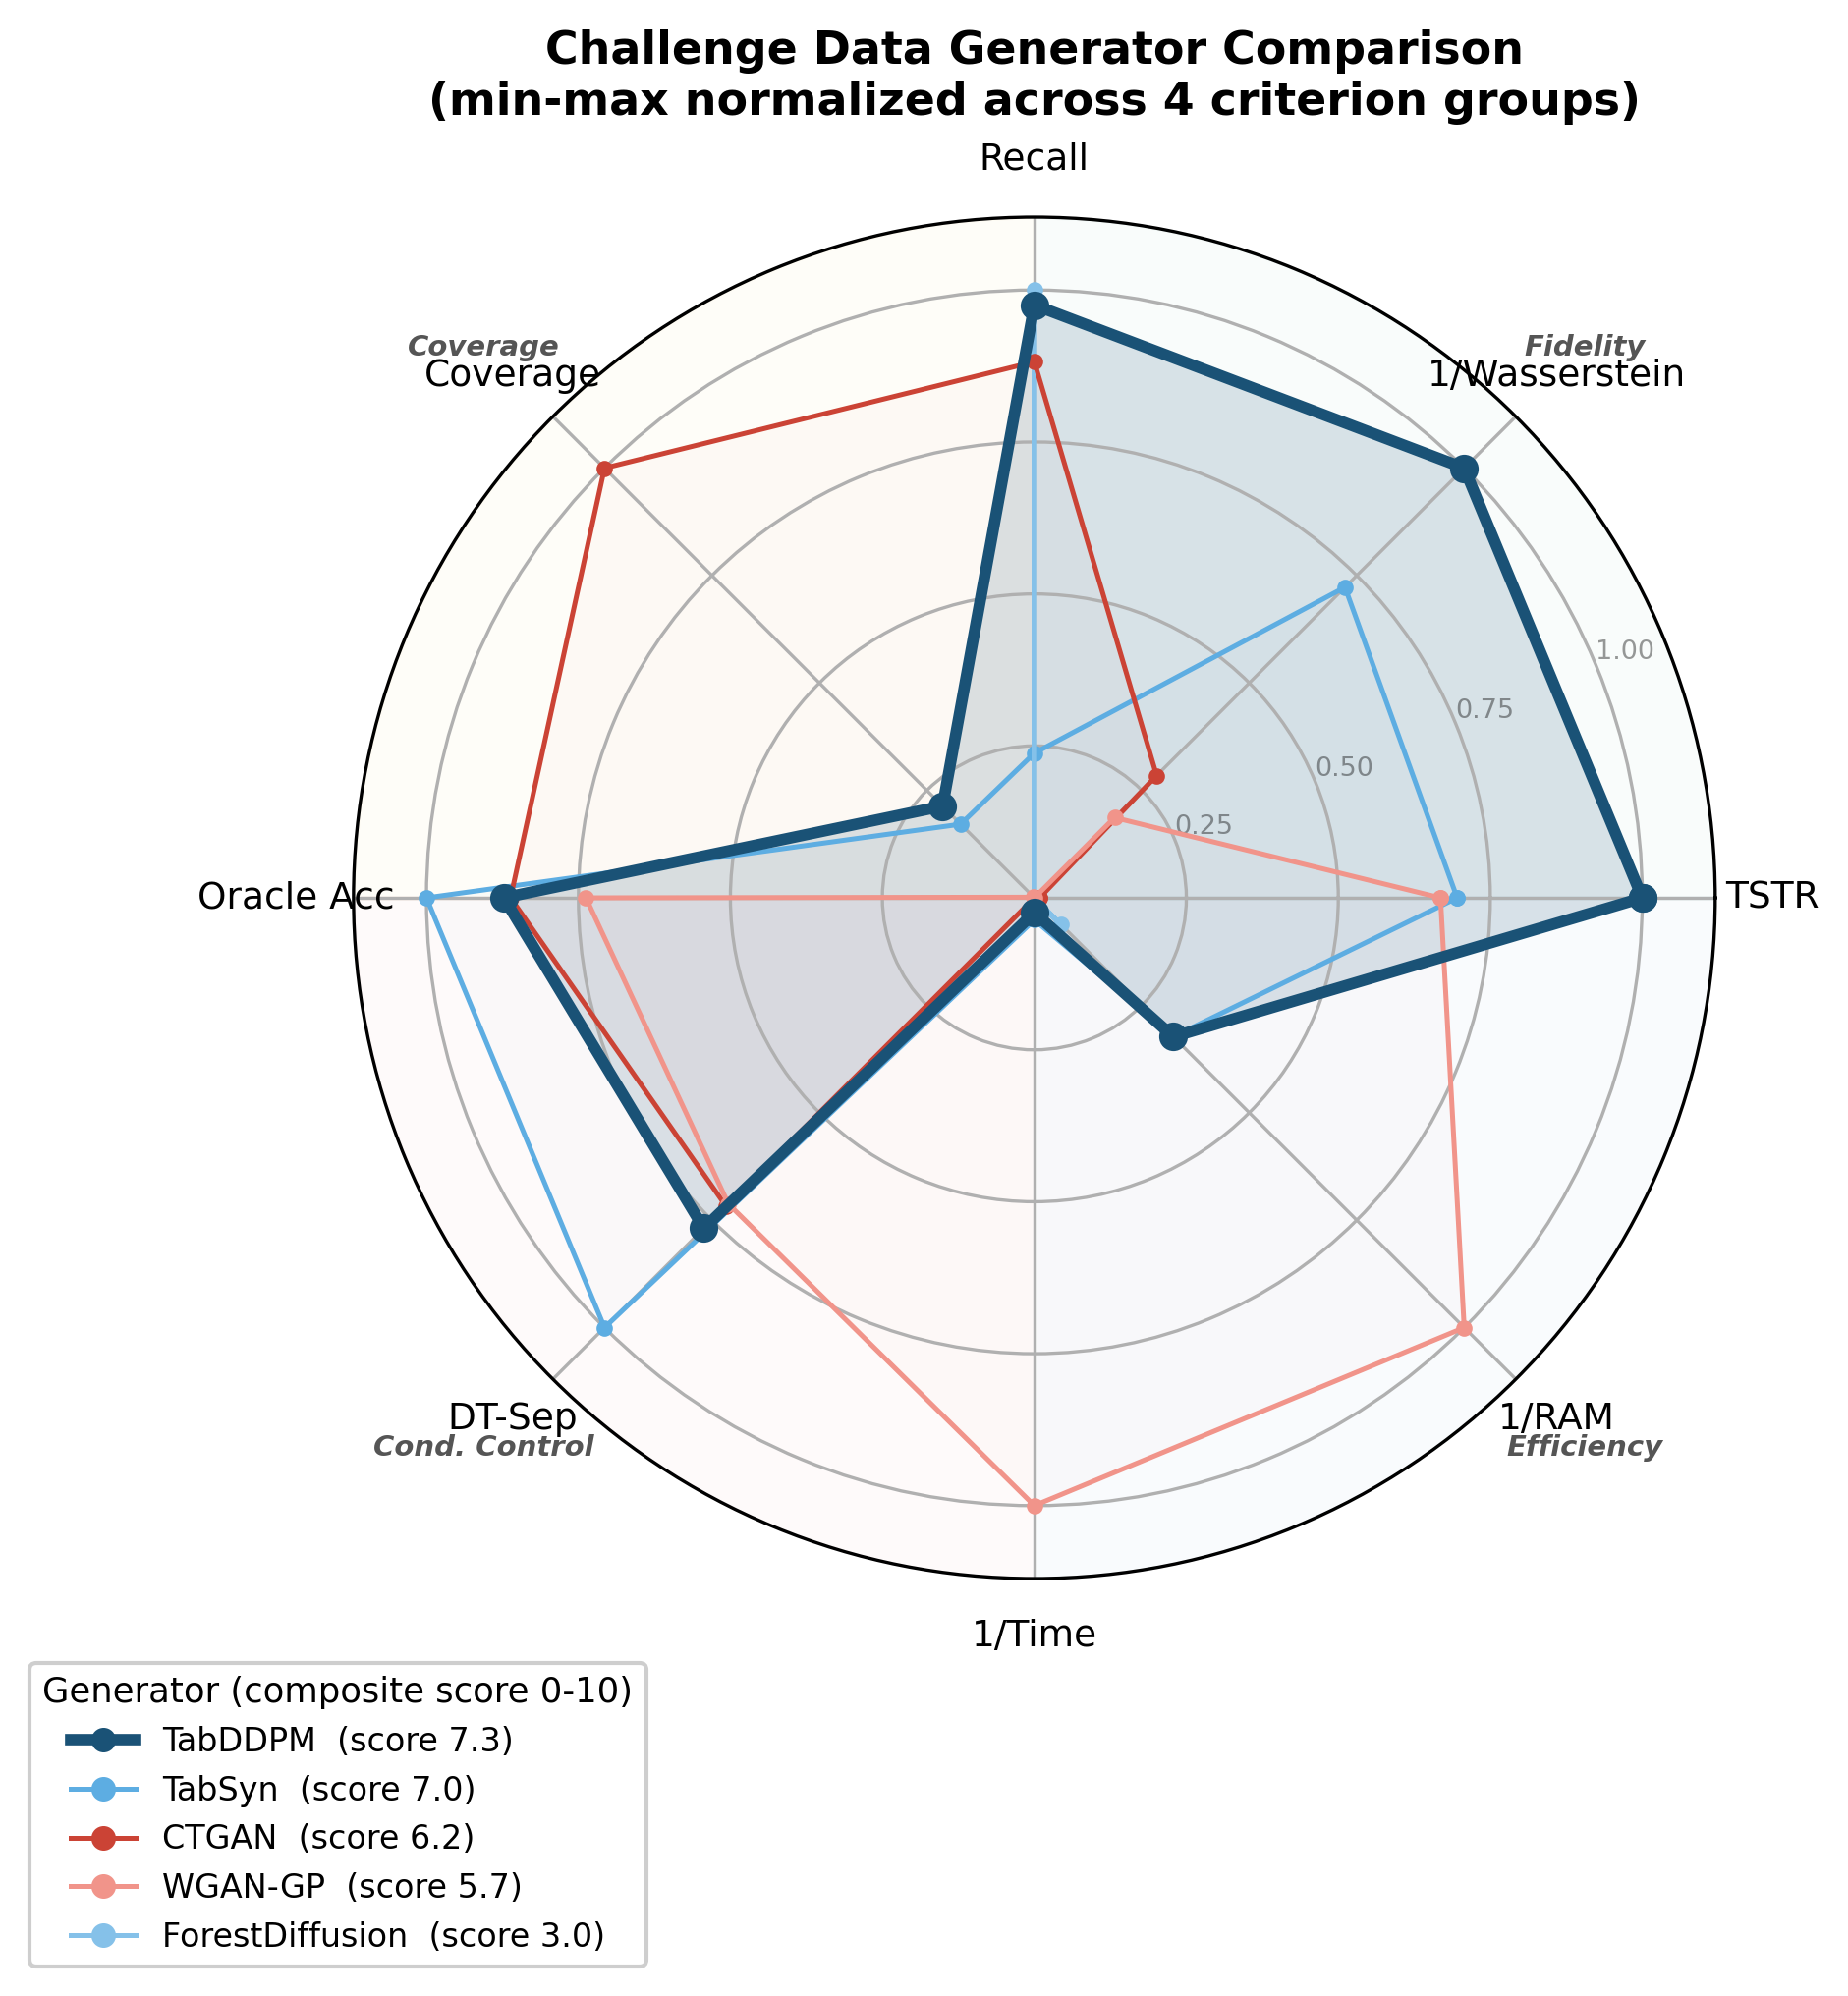
\includegraphics[width=0.85\linewidth]{Figures/fig_5_11_ab_testing_generative_models.png}
    \caption{Kết quả A/B Testing mô hình sinh dữ liệu}
\end{figure}

\subsection{Lý do TabDDPM được chọn}
TabDDPM {[}7{]} được chọn làm bộ sinh mặc định cho DT-Guard dựa trên năm lý do kỹ thuật, mỗi lý do gắn liền với yêu cầu cụ thể của hệ thống:

\textbf{(1)} TSTR cao nhất (71,4\%): đảm bảo challenge data phản ánh thực tế. TSTR (Train on Synthetic, Test on Real) đo hiệu năng của mô hình phân loại được huấn luyện trên dữ liệu tổng hợp khi kiểm tra trên dữ liệu thật. TSTR 71,4\% nghĩa là nếu dùng dữ liệu TabDDPM sinh ra để huấn luyện mô hình IDS, mô hình đó đạt 71,4\% accuracy trên dữ liệu thật, phản ánh sát thực tế. Trong DT-Guard, challenge data đóng vai trò "đề thi" để đánh giá hành vi mô hình. Nếu đề thi không phản ánh đúng phân phối thực, kết quả đánh giá sẽ sai lệch, client tốt có thể bị đánh giá thấp (trùng hợp mẫu challenge khó bất thường) hoặc client xấu được đánh giá cao (trùng hợp mẫu challenge dễ). TSTR cao đảm bảo tính đại diện của challenge data.

\textbf{(2)} Wasserstein Distance thấp nhất (0,061): phân phối sinh sát nhất. Wasserstein Distance đo khoảng cách giữa phân phối dữ liệu sinh và phân phối dữ liệu thật, giá trị càng thấp thì hai phân phối càng giống nhau. Điều này đảm bảo challenge data không chỉ đúng nhãn mà còn đúng phân phối đặc trưng trong mỗi nhãn, tránh hiện tượng sinh ra mẫu có nhãn đúng nhưng giá trị đặc trưng bất thường.

\textbf{(3)} Recall cao: bao phủ đầy đủ các lớp tấn công. Recall cao nghĩa là dữ liệu sinh bao phủ hầu hết các vùng của phân phối thực, không bỏ sót lớp tấn công nào. Điều này quan trọng vì nếu challenge data thiếu một lớp tấn công cụ thể (ví dụ: lớp Backdoor), pipeline sẽ không thể phát hiện client đầu độc nhắm vào lớp đó, client có thể phân loại sai lớp Backdoor nhưng vẫn đạt F1 cao nếu challenge data không chứa mẫu Backdoor.

\textbf{(4)} Training time nhanh (\textasciitilde200 giây): phù hợp tích hợp thực tế. TabDDPM được huấn luyện một lần duy nhất trước khi bắt đầu vòng lặp FL. Với 200 giây huấn luyện, tổng thời gian chuẩn bị (bao gồm cả sinh pre-generated challenge pool) vẫn nhỏ hơn đáng kể so với thời gian huấn luyện một round FL (\textasciitilde8,7 giây $\times$ 20 rounds = 174 giây). So với CTGAN (\textasciitilde1600 giây), TabDDPM tiết kiệm 8 lần thời gian chuẩn bị.

\textbf{(5)} Hỗ trợ conditional sampling: sinh theo nhãn chỉ định. TabDDPM cho phép sinh mẫu với nhãn cụ thể bằng cách thêm thông tin nhãn vào đầu vào mạng neural (class-conditional generation). Khả năng này cho phép tạo challenge data với phân bổ nhãn cân bằng, mỗi lớp có số mẫu tương đương, đảm bảo không có lớp nào bị thiểu số trong "đề thi." Các phương pháp không hỗ trợ conditional generation phải sinh ngẫu nhiên rồi lọc theo nhãn, tốn kém hơn và khó kiểm soát tỉ lệ.

\section{Kịch bản C: Đánh giá tính công bằng và phát hiện free-rider}

\subsection{Thiết lập kịch bản free-rider}
Để đánh giá khả năng phát hiện free-rider của DT-PW, thực nghiệm được tiến hành trên CIC-IoT-2023, đưa 4 free-rider (20\% trong 20 client) vào hệ thống. Free-rider sao chép mô hình toàn cục kèm nhiễu không đáng kể thay vì huấn luyện. Bốn chiến lược tổng hợp trọng số được so sánh: DT-PW, Trust-Score (LUP {[}5{]}), Uniform, và FedAvg.

\subsection{Kết quả so sánh}
DT-PW gán trọng số đúng 0,0 cho tất cả 4 free-rider và phân bổ đều cho 16 client thật (mỗi client 0,0625 = 1/16), đạt accuracy cao nhất 72,97\%. Effort Gate phát hiện 100\% free-rider nhờ prediction divergence gần bằng 0.

Trust-Score (LUP {[}5{]}) tạo ra hiệu ứng ngược: free-rider nhận trọng số 0,2448, cao gấp 188 lần so với client thật chỉ 0,0013. Nguyên nhân là Trust-Score đo khoảng cách tham số đến mô hình toàn cục, free-rider có tham số gần nhất nên được đánh giá "đáng tin" nhất. Hiện tượng "đảo ngược ý nghĩa" này khiến accuracy sụt xuống 46,49\%.

Uniform gán trọng số bằng nhau (0,05) cho tất cả, đạt 72,51\%, gần bằng DT-PW chỉ vì trong kịch bản này free-rider echo mô hình toàn cục nên không gây hại chủ động.

FedAvg gán trọng số theo số mẫu, hiệu quả tương tự Uniform trong kịch bản này.

\begin{figure}[H]
    \centering
    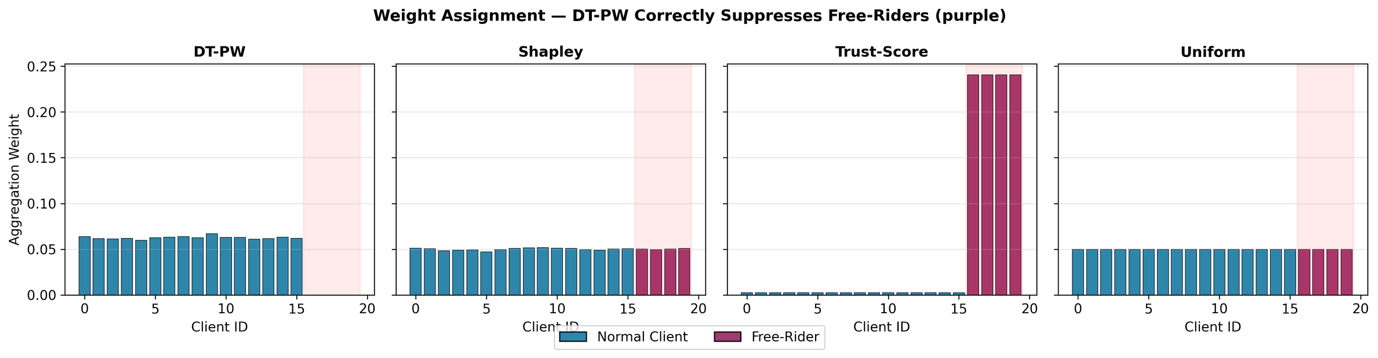
\includegraphics[width=0.85\linewidth]{Figures/fig_5_12_per_client_weight.png}
    \caption{Trọng số per-client theo từng chiến lược tổng hợp}
\end{figure}

\subsection{Phân tích}
Kết quả chứng minh ba điểm quan trọng:

\textbf{(1)} DT-PW là chiến lược duy nhất phát hiện và loại bỏ hoàn toàn free-rider, nhờ đo hành vi suy luận (prediction divergence) thay vì khoảng cách tham số.

\textbf{(2)} Trust-Score dựa trên khoảng cách tham số có lỗ hổng cấu trúc, vô tình thưởng cho free-rider. Đây là bằng chứng mạnh nhất cho thấy chỉ dựa vào đặc trưng tĩnh của tham số sẽ không phản ánh đúng đóng góp thực tế.

\textbf{(3)} DT-PW vừa đảm bảo công bằng vừa cải thiện chất lượng mô hình nhờ ưu tiên client đóng góp tri thức mới.

\section{Phân tích overhead và chi phí tài nguyên}

\subsection{Thời gian thực thi}
DT-Guard có tổng thời gian trung bình mỗi round là 8,735 giây trên CIC-IoT-2023, phân tách như sau:

\begin{itemize}
\item
  \textbf{Training per round:} 8,654 giây (chiếm 99,1\%)
\item
  \textbf{DT verification:} 0,064 giây (chiếm 0,7\%)
\item
  \textbf{DT-PW scoring:} 0,017 giây (chiếm 0,2\%)
\item
  \textbf{Tổng overhead DT-Guard:} 0,081 giây (chiếm \textless{} 1\%)
\end{itemize}

So sánh thời gian aggregation với các baseline: FedAvg 0,001 giây, Krum 0,016 giây, Median 0,037 giây, Trimmed Mean 0,019 giây, GeoMed 0,149 giây, SignGuard 0,018 giây, ClipCluster 0,020 giây, LUP 0,031 giây, PoC 0,004 giây. DT-Guard (0,081 giây) có overhead cao hơn nhưng vẫn ở mức có thể chấp nhận, nhỏ hơn 1\% tổng thời gian round.

\textbf{Phân tích nguyên nhân chi phí từng phương pháp:}

Thời gian aggregation của mỗi phương pháp phản ánh trực tiếp độ phức tạp thuật toán. FedAvg (0,001 giây) là nhanh nhất vì chỉ cần một phép tính trung bình có trọng số trên N vector tham số, thao tác O(N $\times$ d) tuyến tính đơn giản. PoC (0,004 giây) nhanh gần như FedAvg vì MMD$^{2}$ chỉ cần tính kernel distance giữa hai tập tham số, không cần lặp. Krum (0,016 giây) chậm hơn 16 lần FedAvg vì cần tính khoảng cách đôi giữa tất cả N bản cập nhật (O(N$^{2}$ $\times$ d)), rồi với mỗi update tìm k khoảng cách gần nhất, chi phí tăng bậc hai theo số client. SignGuard (0,018 giây) và ClipCluster (0,020 giây) có chi phí tương đương do đều cần tính ma trận khoảng cách (sign-based hoặc cosine) rồi thực hiện phân cụm, MeanShift hoặc Agglomerative.

Trimmed Mean (0,019 giây) cần sắp xếp N vector theo L2 norm rồi cắt hai đầu, chi phí sắp xếp O(N log N). LUP (0,031 giây) chậm hơn do thực hiện hai bước: MAD bounding (tính median và độ lệch tuyệt đối) rồi hierarchical clustering, cần xây dựng dendrogram hoàn chỉnh. Median (0,037 giây) cần sắp xếp theo từng chiều tham số, với d = 39 đặc trưng và số tham số MLP lớn (\textasciitilde90.000 tham số), việc tính trung vị cho từng chiều tạo ra chi phí đáng kể. GeoMed (0,149 giây) là chậm nhất trong các baseline, gần gấp đôi DT-Guard, do giải bài toán Weiszfeld lặp: mỗi bước cần tính khoảng cách từ mọi update đến điểm hiện tại rồi cập nhật, lặp cho đến khi hội tụ. Với dữ liệu Non-IID, điểm khởi tạo xa geometric median khiến cần nhiều vòng lặp hơn.

DT-Guard (0,081 giây) nằm giữa: chậm hơn các baseline thống kê đơn giản nhưng nhanh hơn GeoMed. Chi phí được phân bổ thành DT verification (0,064 giây), chạy inference 200 mẫu $\times$ 20 client qua mạng MLP; và DT-PW scoring (0,017 giây), chạy inference thêm một lần cho mô hình toàn cục rồi so sánh dự đoán. Tuy overhead cao hơn FedAvg 81 lần, nhưng xét trong bối cảnh tổng thời gian round (8,735 giây), 0,081 giây là không đáng kể, và lợi ích thu được (FPR = 0\%, DR 98,3\%, phát hiện 100\% free-rider) hoàn toàn vượt trội so với chi phí tăng thêm.

\begin{figure}[H]
    \centering
    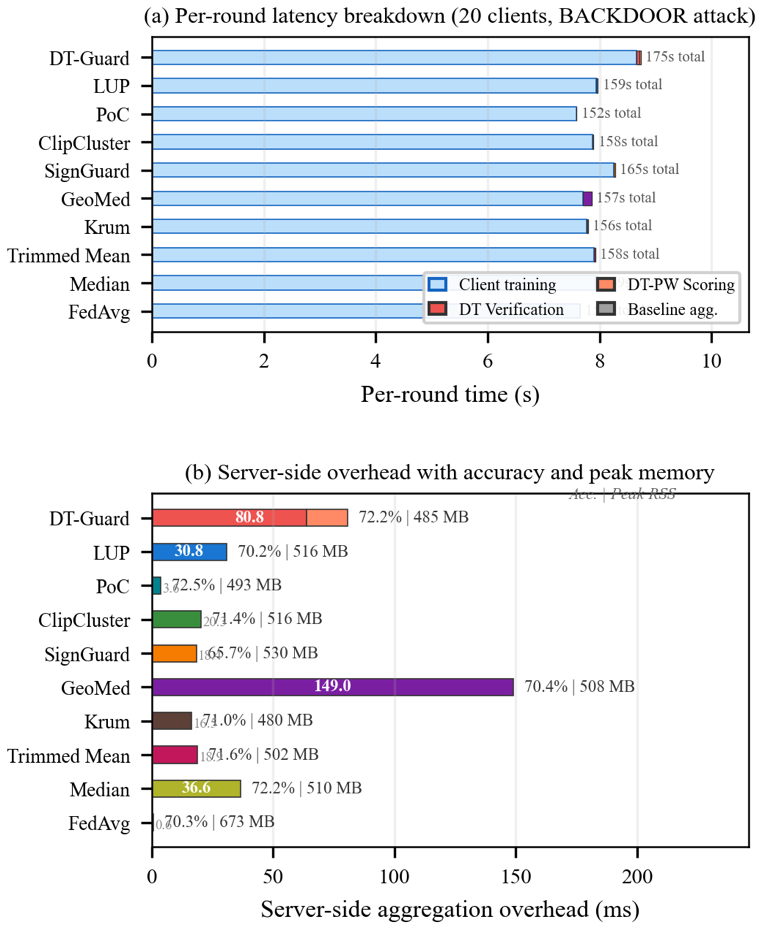
\includegraphics[width=0.85\linewidth]{Figures/fig_5_13_overhead_resource.png}
    \caption{Tổng hợp chi phí tính toán: (a) phân tích thời gian per-round và (b) overhead server-side, accuracy, peak memory theo từng phương pháp}
\end{figure}

\subsection{Bộ nhớ}
Kết quả bất ngờ là DT-Guard có peak memory thấp thứ hai: 485,34 MB, thậm chí thấp hơn FedAvg (673,09 MB). Nguyên nhân là cơ chế sandbox: Digital Twin chỉ nạp một mô hình tại một thời điểm vào bộ nhớ để kiểm thử, rồi giải phóng trước khi nạp mô hình tiếp theo (sequential loading). Trong khi đó, FedAvg và hầu hết baseline phải giữ tất cả bản cập nhật trong bộ nhớ đồng thời.

So sánh peak memory: Krum 479,50 MB, DT-Guard 485,34 MB, PoC 493,05 MB, Trimmed Mean 501,59 MB, GeoMed 507,61 MB, Median 510,28 MB, ClipCluster 515,92 MB, LUP 515,97 MB, SignGuard 530,20 MB, FedAvg 673,09 MB.

\textbf{Phân tích nguyên nhân mức tiêu thụ bộ nhớ:}

Các phương pháp phòng thủ có thể được phân thành hai nhóm theo chiến lược quản lý bộ nhớ. Nhóm 1: Giữ tất cả update đồng thời, bao gồm FedAvg, Trimmed Mean, Median, GeoMed, ClipCluster, LUP, SignGuard. Các phương pháp này cần giữ tất cả N bản cập nhật (mỗi bản \textasciitilde90.000 tham số $\times$ 4 byte = \textasciitilde360 KB) trong bộ nhớ để thực hiện tính toán (sắp xếp, phân cụm, hoặc trung bình). Với N = 20 client, tổng bộ nhớ cho tham số là \textasciitilde7,2 MB, không lớn so với mô hình, nhưng cần thêm các ma trận trung gian cho tính toán (khoảng cách đôi, phân cụm, v.v.). FedAvg có peak memory cao nhất (673 MB) vì ngoài N bản cập nhật, còn giữ bộ đệm cho tính trung bình có trọng số trên toàn bộ tham số. SignGuard (530 MB) cần thêm bộ nhớ cho ma trận sign features (pos/neg/zero cho từng chiều $\times$ N client). LUP và ClipCluster (\textasciitilde516 MB) cần thêm ma trận khoảng cách và dendrogram cho hierarchical clustering.

Nhóm 2: Sequential processing, bao gồm DT-Guard và Krum. Krum có peak thấp nhất (479,5 MB) vì chỉ cần tính khoảng cách từng update đến k update gần nhất, có thể thực hiện tuần tự mà không cần giữ toàn bộ ma trận khoảng cách trong bộ nhớ. DT-Guard (485 MB) thấp hơn đáng kể so với FedAvg nhờ cơ chế sandbox: tại mỗi thời điểm, chỉ có một mô hình client được nạp vào sandbox để chạy inference trên challenge data (200 mẫu), sau đó được giải phóng hoàn toàn trước khi nạp mô hình tiếp theo. Bộ nhớ peak xảy ra khi nạp mô hình + challenge batch + output tensors, nhưng tổng vẫn nhỏ hơn FedAvg vì FedAvg phải giữ tất cả N bản cập nhật đồng thời trong quá trình tính trung bình.

Điểm đáng chú ý là: mặc dù DT-Guard thực hiện nhiều tác vụ hơn (inference 20 client $\times$ 200 mẫu + tính Trust-Score + tính prediction divergence), tổng bộ nhớ vẫn thấp hơn các phương pháp đơn giản hơn. Đây là minh chứng cho hiệu quả của thiết kế sequential loading, đánh đổi thời gian (chạy tuần tự thay vì song song) để giảm bộ nhớ đỉnh, phù hợp với môi trường IoT nơi tài nguyên bộ nhớ hạn chế.

\subsection{Trade-off chi phí - lợi ích}
Để đánh giá toàn diện, cần đặt chi phí tăng thêm của DT-Guard trong ngữ cảnh lợi ích an ninh thu được.

\textbf{Về thời gian:} Chi phí tăng thêm 0,081 giây/round (\textless 1\% tổng thời gian) tương đương với mức overhead thấp nhất có chấp nhận được trong các hệ thống phân tán. Để hình dung, với 20 round FL, tổng thời gian huấn luyện là \textasciitilde175 giây, trong đó overhead của DT-Guard chỉ chiếm \textasciitilde1,6 giây, ít hơn thời gian một epoch huấn luyện cục bộ (\textasciitilde1,4 giây). Trong thực tế, thời gian round FL bị chi phối gần như hoàn toàn bởi huấn luyện cục bộ (99,1\%) và giao tiếp mạng (không đo trong mô phỏng), nên 0,7\% thêm cho verification là không đáng kể.

\textbf{Về bộ nhớ:} DT-Guard không những không tăng peak memory mà còn giảm xuống 485 MB so với FedAvg (673 MB), tiết kiệm 28\% bộ nhớ. Trong môi trường IoT nơi bộ nhớ RAM hạn chế, đây là lợi ích thay vì chi phí.

\textbf{Về lợi ích an ninh, so sánh trực tiếp với chi phí:}

\begin{longtable}[]{@{}
  >{\raggedright\arraybackslash}p{(\linewidth - 10\tabcolsep) * \real{0.1521}}
  >{\raggedright\arraybackslash}p{(\linewidth - 10\tabcolsep) * \real{0.1982}}
  >{\raggedright\arraybackslash}p{(\linewidth - 10\tabcolsep) * \real{0.1699}}
  >{\raggedright\arraybackslash}p{(\linewidth - 10\tabcolsep) * \real{0.1377}}
  >{\raggedright\arraybackslash}p{(\linewidth - 10\tabcolsep) * \real{0.1865}}
  >{\raggedright\arraybackslash}p{(\linewidth - 10\tabcolsep) * \real{0.1556}}@{}}
\caption{Trade-off chi phí - lợi ích giữa DT-Guard và các phương pháp đại diện} \\
\toprule\noalign{}
\begin{minipage}[b]{\linewidth}\centering
\textbf{Phương pháp}
\end{minipage} & \begin{minipage}[b]{\linewidth}\centering
\textbf{Overhead (ms/round)}
\end{minipage} & \begin{minipage}[b]{\linewidth}\centering
\textbf{Peak Memory (MB)}
\end{minipage} & \begin{minipage}[b]{\linewidth}\centering
\textbf{FPR}
\end{minipage} & \begin{minipage}[b]{\linewidth}\centering
\textbf{DR (50\% malicious)}
\end{minipage} & \begin{minipage}[b]{\linewidth}\centering
\textbf{Free-rider}
\end{minipage} \\
\midrule\noalign{}
\endfirsthead
%
\multicolumn{6}{c}{{\textit{(tiếp) Bảng 5.4}}} \\
\toprule\noalign{}
\begin{minipage}[b]{\linewidth}\centering
\textbf{Phương pháp}
\end{minipage} & \begin{minipage}[b]{\linewidth}\centering
\textbf{Overhead (ms/round)}
\end{minipage} & \begin{minipage}[b]{\linewidth}\centering
\textbf{Peak Memory (MB)}
\end{minipage} & \begin{minipage}[b]{\linewidth}\centering
\textbf{FPR}
\end{minipage} & \begin{minipage}[b]{\linewidth}\centering
\textbf{DR (50\% malicious)}
\end{minipage} & \begin{minipage}[b]{\linewidth}\centering
\textbf{Free-rider}
\end{minipage} \\
\midrule\noalign{}
\endhead
\bottomrule\noalign{}
\endlastfoot
FedAvg & 1 & 673 & N/A & Sụp \textless{} 1\% (MPAF) & Không phát hiện \\
GeoMed & 149 & 508 & Cao (LIE) & Sụp (LIE) & Không phát hiện \\
LUP & 31 & 516 & 26,7\% trung bình & 72,2\% accuracy & Thưởng (0,2448) \\
\textbf{DT-Guard} & \textbf{81} & \textbf{485} & \textbf{0\%} & \textbf{98,3\%} & \textbf{Loại (0,0)} \\
\end{longtable}

Bảng trên cho thấy GeoMed có overhead gần gấp đôi DT-Guard (149 ms vs. 81 ms) nhưng lại sụp đổ trước tấn công LIE, chi phí cao hơn mà lợi ích thấp hơn. LUP có overhead thấp hơn DT-Guard (31 ms vs. 81 ms) nhưng FPR 26,7\% và thưởng free-rider, tiết kiệm 50 ms mỗi round đổi với việc loại nhầm hơn 1/4 client lành tính là một sự đánh đổi không thể chấp nhận trong hệ thống thực. DT-Guard chi thêm 50 ms/round so với LUP nhưng thu được FPR = 0\%, DR tăng đáng kể, và phát hiện 100\% free-rider.

Kết luận: tỉ lệ chi phí/lợi ích của DT-Guard là thuận, chi phí tăng thêm (\textless 1\% thời gian, giảm 28\% bộ nhớ) hoàn toàn xứng đáng với lợi ích an ninh đạt được (FPR = 0\%, DR 98,3\%, phát hiện free-rider). Hệ thống có thể triển khai trong môi trường thực tế mà không ảnh hưởng đáng kể đến hiệu năng.

\section{Bàn luận tổng hợp}

\subsection{Tại sao DT-Guard hiệu quả?}
Hiệu quả của DT-Guard bắt nguồn từ kiểm chứng hành vi chủ động thay vì phân tích tham số thụ động. Thực nghiệm xác nhận bốn trường hợp: tấn công dù giữ tham số bình thường nhưng hành vi sai bị phát hiện, client Non-IID dù tham số lệch nhưng hành vi đúng được chấp nhận, và free-rider với prediction divergence gần 0 bị loại. Pipeline 4 lớp đánh giá toàn diện từ nhiều góc nhìn (hiệu năng phát hiện, kháng backdoor, lệch tham số, ổn định), kết hợp với fusion thích ứng và DT-PW tạo ra khả năng phân biệt mà không phương pháp đơn lẻ nào đạt được.

\subsection{Tại sao FPR = 0\%?}
FPR = 0\% là kết quả quan trọng nhất. Các phương pháp thụ động đo khoảng cách tham số: client có tham số lệch xa bị loại. Trong môi trường Non-IID, client lành tính có dữ liệu thiên lệch tự nhiên bị nhầm là tấn công. DT-Guard giải quyết nhờ kiểm chứng hành vi: client Non-IID lành tính dù tham số lệch nhưng phân loại chính xác trên challenge data $\rightarrow$ IDS Performance Score cao $\rightarrow$ vượt Trust Gate. Cơ chế fusion thích ứng đóng vai trò then chốt: trong balanced mode, IDS Performance Score (trọng số 0,7) bù cho Parameter Similarity Score thấp (trọng số 0,3).

\subsection{So sánh trực tiếp với LUP}
LUP {[}5{]} là phương pháp gần nhất về hiệu năng tổng thể, nhưng có hai hạn chế cấu trúc: (1) FPR cao (trung bình 26,7\% tại 50\% malicious) do đo khoảng cách tham số; (2) Thưởng free-rider (0,2448 vs 0,0013 cho client thật) do Trust-Score dựa trên khoảng cách. DT-Guard giải quyết cả hai vấn đề nhờ kiểm chứng hành vi và prediction divergence.

\subsection{Các hạn chế nhận diện được}
Mặc dù kết quả khả quan, DT-Guard có một số hạn chế: (1) Overhead tăng tuyến tính theo số client, với hệ thống rất lớn cần tối ưu thêm bằng parallel verification hoặc sampling; (2) Phụ thuộc chất lượng TabDDPM, nếu domain thay đổi (concept drift) mà không retrain bộ sinh, chất lượng verification giảm; (3) Chưa thử nghiệm trên mạng IoT thực tế quy mô lớn.

\section{Tổng kết chương}
Thực nghiệm trên CIC-IoT-2023 và ToN-IoT cho thấy DT-Guard duy trì accuracy ổn định, DR đạt 98,3\% (CIC-IoT-2023) và 99,5--100\% (ToN-IoT) ở 50\% malicious, FPR 0\% trên cả 5 loại tấn công ở cả hai dataset; TabDDPM đạt TSTR cao nhất (71,4\%) và Wasserstein Distance thấp nhất (0,061); DT-PW phát hiện 100\% free-rider. Overhead 80,8 ms/round (\textless 1\%) và peak memory 485 MB (thấp nhất). Kết quả này tạo nền tảng cho Chương 6.
